\documentclass[conference]{IEEEtran}
\IEEEoverridecommandlockouts
% The preceding line is only needed to identify funding in the first footnote. If that is unneeded, please comment it out.
\usepackage{cite}
\usepackage{amsmath,amssymb,amsfonts}
\usepackage{algorithmic}
\usepackage{graphicx}
\usepackage{textcomp}
\usepackage{hyperref}
\usepackage[ruled,vlined]{algorithm2e}
\usepackage{enumitem}
\usepackage{booktabs}
\usepackage[font=small,skip=0pt]{caption}
\hypersetup{
    colorlinks=true,
    linkcolor=blue,
    filecolor=magenta,      
    urlcolor=blue,
}
\usepackage{xcolor}
\def\BibTeX{{\rm B\kern-.05em{\sc i\kern-.025em b}\kern-.08em
    T\kern-.1667em\lower.7ex\hbox{E}\kern-.125emX}}
\begin{document}

\title{Musical Genre Classification and Comparison Using Different Classifiers\\
{\footnotesize \textsuperscript{}}
\thanks{}
}

\author{\IEEEauthorblockN{1\textsuperscript{st} Giuseppe Bonura}
\IEEEauthorblockA{\textit{University of Milan} \\
\textit{Department of Computer Science}\\
Italy, Milan \\
giuseppe.bonura@studenti.unimi.it}
}

\maketitle

\begin{abstract}
The automatic classification of musical genres is a complex operation and the features available are many. This study are divide in two parts, in the first, the k-means algorithm was used to determine the space of the features, subsequently were analyzed time and frequency features, compared, chosen and used with various classification algorithms in order to analyze their performance.
\end{abstract}

\begin{IEEEkeywords}
Classification, Feature Extraction, Ensemble of classifiers, MLP, SVM, K-Means, Random Forest,
Musical Genre Classification.
\end{IEEEkeywords}

\section{Introduction}
\noindent
Since ancient times, humans has made use of classification, that is, the activity that consists in arranging the entities of a given domain of knowledge a) People of a given social group, b) Animal or plant species and c) Objects of a certain kind, in suitable containers of knowledge between which links are established regarding one or more relationships. This classification can also be applied in the musical field, specifically on one of the many properties that distinguish an audio sample, the \textbf{"genre"}\cite{Genre}. A musical genre is represented by a label created and used by humans to categorize and describe the large universe of music. Taken together, musical genres don't have very precise and rigorous definitions but emerge as a result of a complex interaction between the public, marketing, historical and cultural factors.
The automatic classification of musical genres has turned out to be a complex task from the earliest studies. The different characteristics that allow to identify a genre are different, in addition to those mentioned above, we can consider harmonic and rhythm as determining factors. Over the years, thanks to the evolution of the study of signals, it has been possible to implement functions capable of extracting these characteristics, which we will divide into two categories Time Domain Features and Frequency Domain Features. The importance of systems capable of automatically recognizing musical genres has had a certain relevance, especially in recent years, thanks to the increase in systems for using digital content online, and streaming/purchasing service such as spotify, deezer, soundcloud. We can place the recognition of musical genres in applications capable of performing music auto-tagging, automatically catalog music within huge databases and automatically create playlists according to some parameters provided by the user. In the literature there are many papers related to music classification, one of the first studies conducted by Tzanetakis and Cook in 2002 \cite{1021072} involved using of both the mixture of Gaussian model and k-nearest neighbors along with three sets of carefully hand-extracted features representing timbral texture, rhythmic content and pitch content. Another study conducted by Tao Li and George Tzanetakis \cite{1285840} who plans to take part in the study of Tzanetakis and Cook using different combinations of features and apply different classifiers obtaining better accuracy's. The study conducted in this document involves the use of a clustering algorithm known as K-Means to be able to determine the space of the features, also verifying through the Silhouette method the interpretation and validation of consistency within clusters of data \cite{ROUSSEEUW198753}. The technique provides a succinct graphical representation of how well each object has been classified. Exploits the approaches used in the two papers cited, i.e. the extraction of multiple types of features, divided into two groups, Time Domain Features and Frequency Domain Features.
These features were then combined and fed to multiple classifiers of different types, specifically a deep multi-layer perceptron network, an ensemble learning method known as random forest and in finally another supervised learning models called Support-Vector Machine or SVM. This approach was used to show with scientific evidence that not all features are necessary during multi-label classification, but that on the contrary, techniques can be exploited to reduce the number of features and therefore the computation complexity of the model. Furthermore, to provide objective feedback on the performance of some classifiers, and that not always the most complex can lead to the best result.
\begin{figure*}
    \centering
    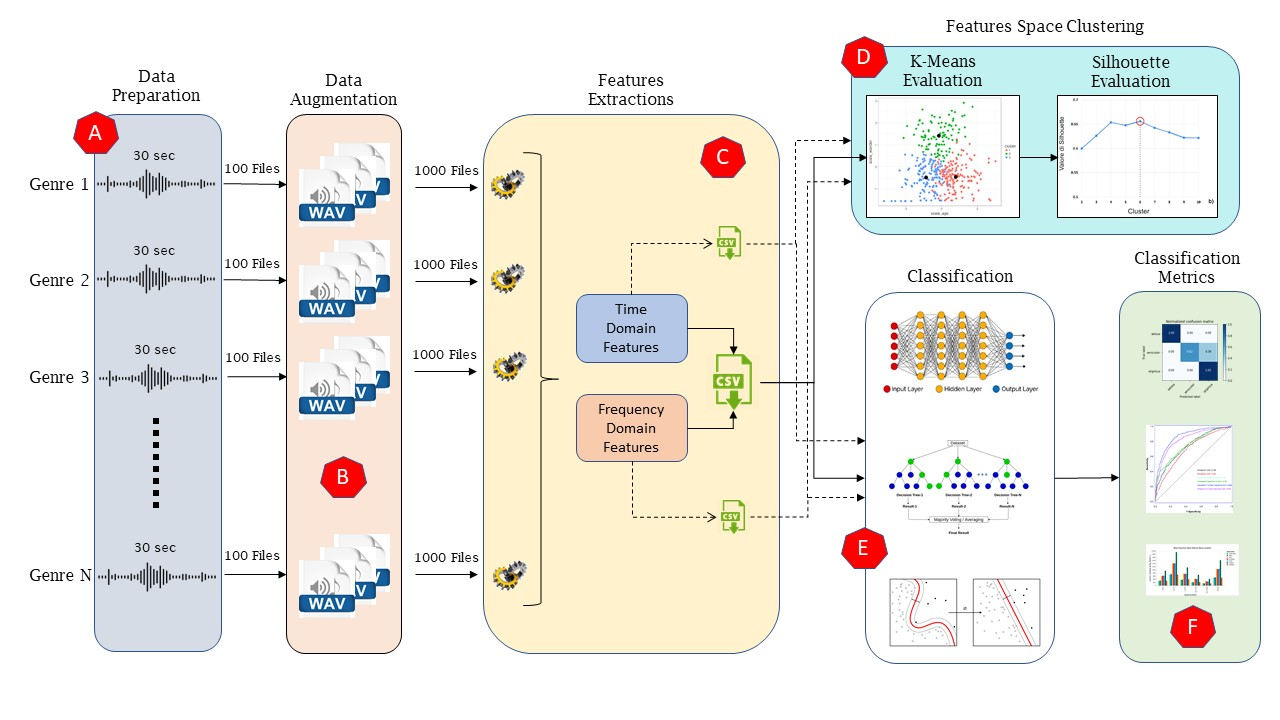
\includegraphics[width=16cm]{Image/System_Overview.jpg}
    \caption{\label{fig:FirstArchitecture}High level architecture for music genres classifications system.}
\end{figure*}

\section{System Overview}
\noindent
The architecture of the implemented system is basically divided into 6 blocks, in the first two we have sample data preparation and data augmentation. The heart of the system is located in the third step or the extraction of the features and their choice. Next we have the clustering of the features and the classification through various approaches. As a last step we have the evaluation of the obtained results.

\subsection{Data Preparation}
\noindent
As a first approach to the problem, after having identified the data set of interest \href{http://marsyas.info/downloads/datasets.html}{GTZAN}, based on this we have created our data-set choosing from various albums and compilations of various years for each musical genre that wee are chose to considered. 
\subsection{Data Augmentation}
\noindent
There are a lot techniques for audio data augmentations, in this project we used one of the most simple, or split data in more sub samples for increase the number of data that. Starting from 100 samples of 30 seconds and reaching 1000 samples of 3 seconds.
\subsection{Features Extraction}
\noindent
Feature extraction is the process of computing a compact numerical representation that can be used to characterize a segment of audio. The design of descriptive features for a specific application is the main challenge in building pattern recognition systems. Once the features are extracted standard machine learning techniques which are independent of the specific application area can be used.\cite{1021072}
\begin{enumerate}
    \item Time Domain Features
    \begin{enumerate}
        \item\textbf{Tempo}: Particularly useful features to extract from musical sources may be an approximation of tempo as well as the beat onset indices, an array of frame numbers corresponding to beat events.
        \item\textbf{Energy}: This feature provides the so-called power of the signal. Let ${s_i(k)}$, where $k=1...W_L$ be the sequence of audio samples of the ${i_t}_h$ frame, where $W_L$ is the length of the frame. The short-term energy is computed according to the equation:
        \begin{equation}\label{eq:energy}\small
            E(i)=\frac{1}{W_L}\cdot\sum_{n=1}^{W_L} {s_i(n)}^2\cdot
        \end{equation}
        \item\textbf{Energy Entropy}: The entropy of energy can be interpreted as a measure of abrupt changes in the energy level of an audio signal. In order to compute it, we first divide each short-term frame in $K$ sub-frames of fixed duration. Then, for each sub-frame, $j$,we compute it's energy as in Eq.\ref{eq:energy} and divide it by the total energy. At a final step, the entropy,${H_i}$ of the sub-frames sequence is computed according to the equation:
        \begin{equation}\label{eq:entropy_energy}\small
            H(i)=-\sum_{j=1}^{W_L} e_j\cdot\log_{2}(e_j)\cdot     
        \end{equation}
        \item\textbf{Root Mean Square Energy (RMSE)}:
        Root-Mean-Square Energy is typically denoted RMS energy, is another time domain feature, computed as shown in Eq.\ref{eq:rmse} where $W_L$ represents frame size, i.e., the number of samples in each frame and ${s_i(k)}$ the signal. As it relates to perceived sound intensity, RMS energy can be used for loudness estimation and as an indicator for new events in audio segmentation. \cite{rmse}
        \begin{equation}\label{eq:rmse}\small
            RMSE=\sqrt{\frac{1}{W_L}\cdot\sum_{n=1}^{W_L} {s_i(n)}^2\cdot}
        \end{equation}
        \item\textbf{Zero-Crossing Rate (ZCR)}: Measures the number of times the amplitude value changes it's sign. In other words, the number of times the signal changes value, from positive to negative and vice versa, divided by the length of the frame, according to the equation:
        \begin{equation}\label{eq:zcr}\small
            Z(i)=\frac{1}{2W_L}\cdot\sum_{n=1}^{W_L} |sgn[s_i(n)]-sgn[s_i(n-1)]|\cdot
        \end{equation}
    \end{enumerate}
    \item Frequency Domain Features
    \begin{enumerate}
        \item\textbf{Spectral Centroid}: The spectral centroid is a measure to characterize the "center of mass" of a given spectrum. Perceptually, it has a robust connection with the impression of sound brightness, or rather as an indication of the amount of high-frequency content in a sound, obtained according to the following equation, where $m_t(n)$ represents number of frequency bins, i.e., the number of the highest frequency band.
        \begin{equation}\label{eq:spectral_centroid}\small
            SC_i=\frac{\sum_{k=1}^{N} m_t(n)\cdot n}{\sum_{n=1}^{N} m_t(n)}
        \end{equation}
        \item\textbf{Spectral Bandwidth}: Spectral bandwidth is derived from the spectral centroid and indicates the spectral range of the interesting parts in the signal, i.e., the parts around the centroid. It can be interpreted as variance from the mean frequency in the signal. The definition is given in Eq.\ref{eq:spectral_bw}.The average bandwidth of a music piece may serve to describe its perceived timbre.\cite{Lerch:1540227}
        \begin{equation}\label{eq:spectral_bw}\small
            BW_i=\frac{\sum_{n=1}^{N} |n-SC_i|\cdot m_t(n)}{\sum_{n=1}^{N} m_t(n)}
        \end{equation}
        \item\textbf{Spectral Contrast}: Four each frame of a spectrogram $s$ is divided into sub-bands. For each sub-band, the energy contrast is estimated by comparing the mean energy in the top quantile (peak energy) to that of the bottom quantile (valley energy). High contrast values generally correspond to clear, narrow-band signals, while low contrast values correspond to broad-band noise.\cite{1035731}
        \item\textbf{Spectral Rolloff}: This feature is defined as the frequency below which a certain percentage (usually around 85-90\%) of the magnitude distribution of the spectrum is concentrated.
        Therefore, if the ${m_t}_h$ DFT coefficient corresponds to the spectral rolloff of the ${i_t}_h$ frame, then it satisfies the following Eq. \ref{eq:spectral_rolloff}, where C is the adopted percentage (user parameter). The spectral rolloff frequency is usually normalized by dividing it with N, so that it takes values between 0 and 1.
        \begin{equation}\label{eq:spectral_rolloff}\small
            \sum_{n=1}^{m} m_t(n) = C\cdot \sum_{n=1}^{N} m_t(n)
        \end{equation}
        \item\textbf{Mel Frequency Cepstral Coefficient}: Mel frequency cepstral coefficients (MFCCs) have their origin in speech processing but were also found to be suited to model timbre in music. The MFCC feature is calculated in the frequency domain, derived from the signal’s spectrogram and for each frame, cepstral coefficients are computed using Mel-filter bank with a variable numbers of Mel filters. In music signal processing, between 13 and 25 MFCCs are typically computed for each frame. The MFCC feature extraction for this project can be summarized in five points\cite{mfccs}:
        \begin{itemize}
          \item\textbf{Pre-emphasis.}
          \item\textbf{Frame blocking and windowing.}
          \item\textbf{DFT spectrum.}
          \item\textbf{Mel spectrum.}
          \item\textbf{Discrete cosine transform (DCT).}
        \end{itemize}
        \item\textbf{Chromogram}: In music, the term chromagram is attentive to the twelve different pitch classes. This vector of features is computed by grouping the DFT coefficients of a short-term window into 12 bins. Each bin represents one of the 12 equal tempered pitch classes of Western-type music. Each bin produces the mean of log-magnitudes of the respective DFT coefficients. One main characteristic features of colour is that they capture the harmonic and melodic features of music, at the same time robust to changes in timbre and instrumentation.
        \item\textbf{Constant-Q chromagram}: The frequencies that have been chosen to make up the scale of Western music are geometrically spaced. Thus the DFT, although extremely efficient in the FFT implementation, yields components which do not map efficiently to musical frequencies. This is because the frequency components calculated with the DFT are separated by a constant frequency difference and with a constant resolution. A calculation similar to a DFT but with a constant ratio of center frequency to resolution has been made; this is a constant Q transform and is equivalent a 1/24-oct filter bank. In addition to advantages for resolution, representation with a constant pattern has the advantage that note identification, instrument recognition, and signal separation.\cite{costant_q}
        \item\textbf{Chroma Energy Normalized}: That there are different ways of computing chroma features and that the properties of chroma features can be adjusted by applying suitable post processing steps such as logarithmic compression, normalization, or smoothing. The two steps, quantization and smoothing, amount to computing weighted statistics of the energy distribution over a window of $l$ consecutive vectors. Therefore, we call the resulting features CENS. The main idea of CENS features is that taking statistics over relatively large windows smooths out local deviations in tempo, articulation, and execution of note groups such as trills or arpeggios.\cite{cens}
    \end{enumerate}
\end{enumerate}

\subsection{Features Space Clustering}
\noindent
In this architecture block, after extracting the characteristics from the audio samples we applied an unsupervised learning technique. It too, as in any classification problem, tries to learn in order to associate a label y of the set Y with a given point x of the input space X, in our case the correct musical genre. The substantial difference between unsupervised and supervised learning techniques is that of automatically extracting knowledge from the input data. This knowledge is extracted without specific knowledge of the content to be analyzed. One of the main algorithms of this category is the clustering algorithm called K-Means. The aim of the K-means algorithm is to minimize the total inter-cluster variance and to maximize the intra-cluster variance. We first choose K initial centroids, where K is a user specified parameter, namely, the number of clusters desired. Each point is then assigned to the closest centroid basis of a predetermined measure of similarity or distance, and each collection of points assigned to a centroid is a cluster. The centroid of each cluster is then updated for each iteration based on the points assigned to the cluster, until the algorithm converges.
\begin{figure}[!ht]
    \centering
    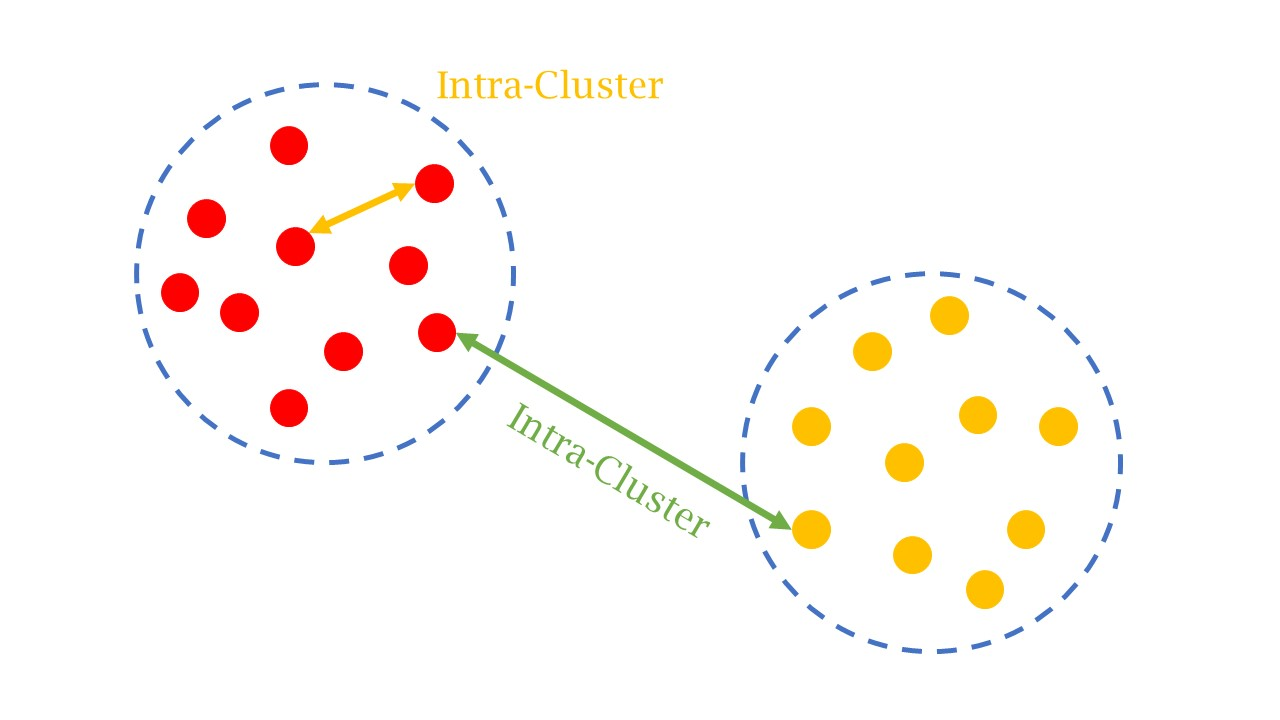
\includegraphics[width=0.9\linewidth]{Image/Intra_Inter.jpg}
    \caption{\label{fig:Intra_Inter_Kmeans}Schematic example of intra-cluster and inter-cluster distance.}
\end{figure}
\newline Now we see depicted below a pseudo code version of the K-Means algorithm:
\begin{algorithm}\small
    \SetAlgoLined
    \SetNlSty{texttt}{[}{]}
    \SetAlgoNlRelativeSize{0}
    \SetNlSkip{0em}
    \nl\KwIn{Set N patterns $x_i$, desired number of clusters K}
    \nl\KwOut{Set of K clusters}
    \nl\emph{Choose K patterns as the $c_j$ centers of clusters}\;
    \nl\Repeat{Convergence criterion are satisfied}
    {
        \nl\emph{Assign each pattern $x_i$ to the cluster $P_i$ that has the center $c_j$ closest to $x_i$ (that is, the one that minimizes d ($x_i$, $c_j$))}\;
        \nl\emph{Recalculate the $c_j$ centers of the clusters using the patterns that belong to each cluster (mean or centroid)}\;
    }
    \nl\KwRet{}
    \caption{K-means}
\end{algorithm}

\subsection{Classification\label{K_Means_pseudo}}
\noindent
The fifth block is dedicated to the classification of the characteristics extracted with the aid of a different supervised classification methods. The ones we have decided to use to be able to compare them are three, we'll see the main peculiarities of each one.
\begin{enumerate}
    \item\textbf{Support Vector Machine}: Support vector machines have shown superb performance at binary classification tasks and handle large dimensional feature vectors better than other classification methods. Basically, a Support Vector Machine aims at searching for a hyper-plane that separates the positive data points and the negative data points with maximum margin. To extend SVM for multi classification there are two approaches called:
    \begin{itemize}
        \item One-Vs-Rest (ovr): Is a heuristic method for using binary classification algorithms for multi-class classification. It involves splitting the multi-class data set into multiple binary classification problems. This approach requires that each model predicts a class membership probability or a probability-like score. The max of these scores is then used to predict a class.\cite{murphy2012machine}
        \item One-Vs-One (ovo): Like ovr, ovo splits a multi-class classification data set into binary classification problems. Unlike ovr that splits it into one binary data set for each class, the ovo approach splits the data set into one data set for each class versus every other class. This is significantly more data sets, and in turn, models than the ovr strategy described in the previous section. The formula for calculating the number of binary data sets, is as follows: ${K \cdot (K-1)}/2$.\cite{murphy2012machine}
    \end{itemize}
    \item\textbf{Random Forest}: The random forest algorithm is an extension of the bagging method as it utilizes both bagging and feature randomness to create an uncorrelated forest of decision trees. Feature randomness, also known as feature bagging generates a random subset of features, which ensures low correlation among decision trees. After several data samples are generated, these models are then trained independently,  producing a more accurate estimate. This is a key difference between decision trees and random forests. While decision trees consider all the possible feature splits, random forests only select a subset of those features.
    \item\textbf{Deep Neural Network}: An artificial neural network (ANN)is a mathematical model that tries to simulate the functioning of neurons present in biological organisms. These models are directly inspired by the functioning of the brain. Neural networks (NN) are made up of a layer of input and output neurons, and possibly one or more intermediate layers called hidden, and if a number of hidden layer is greater than 1 the suffix deep will be prefixed to the network. The interconnections go from one layer to the next and the signal values can be both discrete and continuous. The values of the weights associated with the inputs of each node can be static or dynamic in such a way as to adapt the behavior of the network based on variations in the input signals. The functioning of a NN can be schematized in two phases: the learning phase and the recognition phase. In the learning phase the network is instructed on a sample of data taken from the set of those that will then have to be processed; in the recognition phase, which is then that of normal operation, the network is used to process the incoming data based on the configuration achieved in the previous phase.
\end{enumerate}

\subsection{Classification Metrics}
\noindent
In this section we analyze how to evaluate the goodness of a model or several classification models. The methods used are, the ROC curves and the confusion matrix.
\begin{itemize}
    \item\textbf{Confusion Matrix}: A classifier can be described as a function that maps the elements of a set into certain classes or groups. In the case of supervised classification, the set of data to be classified contains a subdivision into classes, with respect to which it's possible to evaluate the quality of the result produced. In a binary classification problem, the set of data to be classified is divided into two classes that we can conventionally indicate as positive \textbf{(p)} or negative \textbf{(n)}. The results of applying a binary classifier fall into one of the following four categories.
    \begin{enumerate}\small
        \item True Positive (TP).
        \item False Positive (FP).
        \item True Negative (TN).
        \item False Negative (FN).
    \end{enumerate}
    \vspace{5mm} %5mm vertical space
    \item\textbf{ROC Curve}: The classification model would be optimal if it maximized both sensitivity and specificity at the same time. However, this isn't possible. Given the definitions of specificity and sensitivity, we have that, raising the value of specificity, the false positives decreases, but false negatives increase, which leads to a decrease in sensitivity. It can be observed that therefore there is a trade-off between these two parameters, which leads to more sensitive but less specific and, vice versa. Generally the optimal classification corresponds to the point closer to the upper left corner, representing a sensitivity and specificity of 100\%. The curve below is called the ROC curve.
    \begin{equation}\label{eq:sensitivity}\small
        sensitivity=\frac{TP}{TP+FN}    
    \end{equation}
    \begin{equation}\label{eq:specificity}\small
        specificity=\frac{TN}{TN+FP}    
    \end{equation}
    \begin{figure}[!ht]
    \centering
    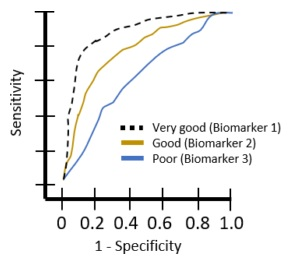
\includegraphics[width=0.7\linewidth]{Image/ROC_V2.jpg}
    \caption{\label{fig:ROC}Example of ROC curve.}
\end{figure}
\end{itemize}

\section{Experimental Results}
\noindent
The first thing during the practical construction of the project was to find various musical albums and collections of 10 genres from various vintages. This operation was necessary in order to populate the data set with sufficient variability. The first script used he's able to divide each audio track into many sub samples of 30 seconds each, then through a second script 100 samples were chosen randomly. In order to increase the amount of data available to us while keeping the extraction of features low at the computational level, the 30-second samples were divided into 10 3-second samples, thus obtaining 1000 3-second samples. The next step in the creation of the data set was the one related to the construction of the script used to extract the characteristics from the audio samples to insert them into a CVS file. The extraction took place using the Librosa library as a support while the two functions for energy extraction and energy entropy were written from scratch. Once the file containing the characteristics of each sample was obtained, the approach we chose to use was to compare the two types of classifications, unsupervised and supervised considering combinations of features and variable number of MFCCs coefficients (13, 20, 40):
\vspace{2mm} %2mm vertical space
\begin{itemize}
    \item Time Domain Features
    \item Frequency Domain Features
\end{itemize}
\vspace{2mm} %2mm vertical space

\noindent
For the extraction of the features, were used the following parameters:
\vspace{2mm} %2mm vertical space
\begin{itemize}\small
    \item Sample Length: 3 sec
    \item Sample Rate: 22050 Hz
    \item Length of the FFT window: 2048
    \item Hop Length: 512
    \item Window Function = Hann 
\end{itemize}
\vspace{2mm} %2mm vertical space

\noindent
For the evaluation of the two classification methodologies (unsupervised and supervised), two scripts in python have been created respectively. Through the aid of third-party libraries and specially created functions were able to conduct a careful evaluation of various models. Let's see the sequential steps performed for the two approaches:
\begin{itemize}\small
    \item Unsupervised Learning:
    \begin{enumerate}
        \item Load data.
        \item Calculate correlation matrix.
        \item Run K-Means algorithm.
        \item Use PCA algorithm for reduce dimensionality.
        \item Plot clusters and centroids on 2D matrix.
        \item Plot confusion matrix.
        \item Plot ROC curve.
        \item Calculate consistency using Silhouette.
    \end{enumerate}
    \item Supervised Learning:
    \begin{enumerate}
        \item Load data.
        \item Split data for train and test.
        \item Calculate correlation matrix.
        \item Use PCA for plot features on 2D matrix.
        \item Plot BPM graph.
        \item Load models.
        \item Evaluate model and get results.
    \end{enumerate}
\end{itemize}

\noindent
After having launched the scripts for the two classification methodologies, we have created appropriate graphs and tables to be able to compare the results obtained.

\begin{figure}[!ht]
    \begin{center}
        \small\textbf{ROC results curves for time features}\par\medskip   
        \begin{minipage}[t]{.24\textwidth}
            \centering
            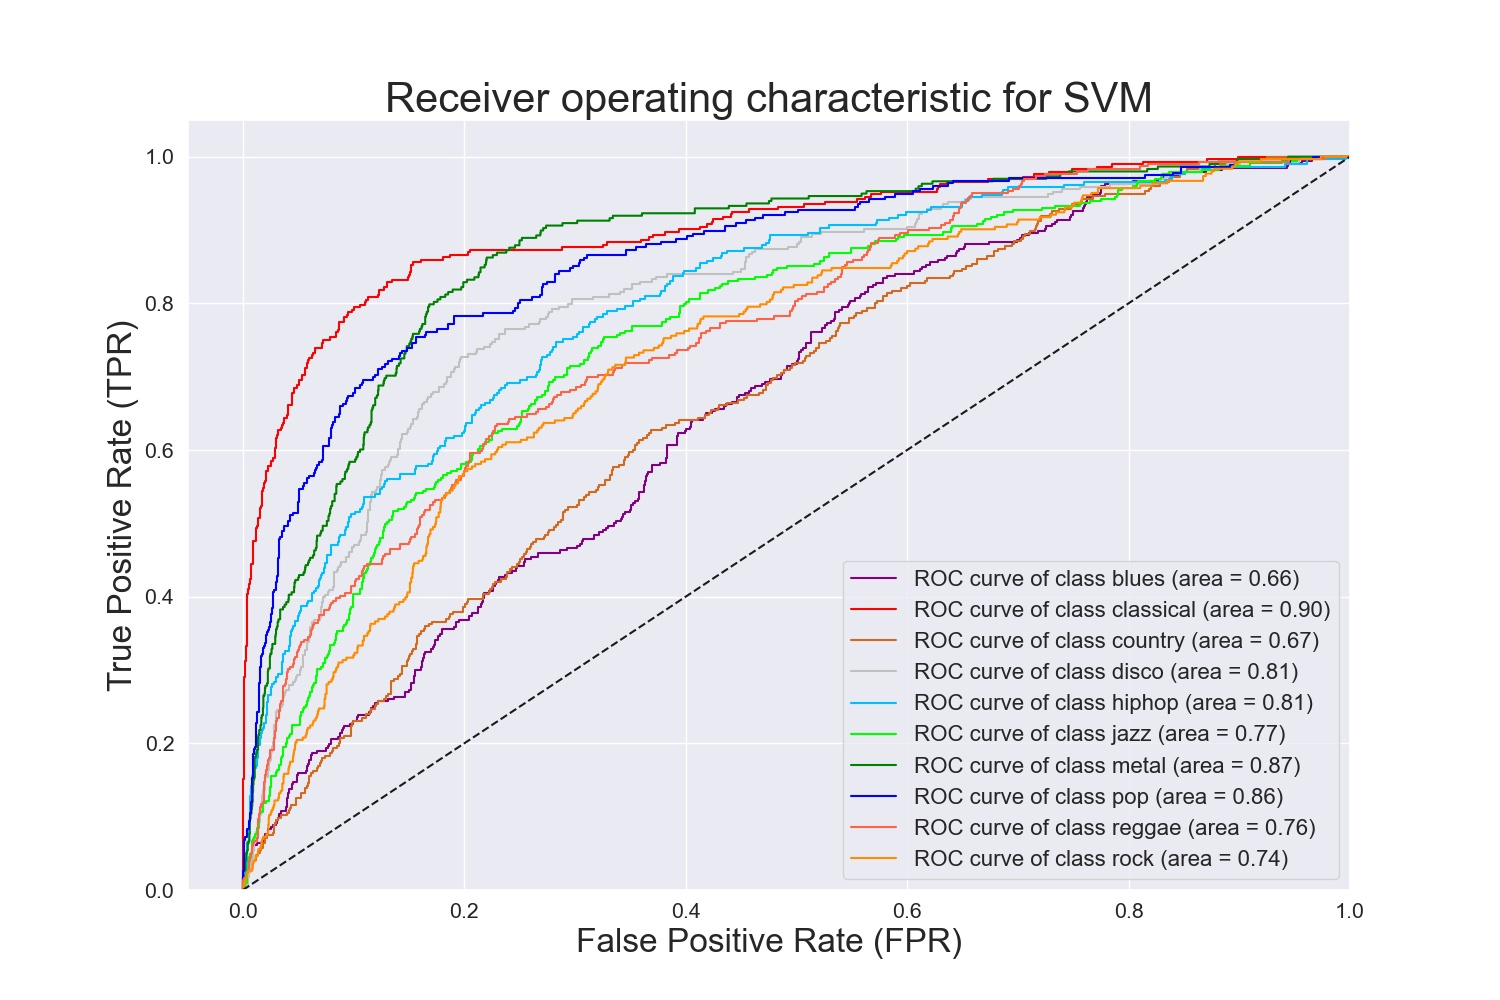
\includegraphics[width=\textwidth]{plot/SL/time_features/SVM_10000_10GEN_GTZAN - ROC Plot.jpg}
            \caption{SVM Time Features}
            \label{fig:SVM Time Features}
        \end{minipage}
        \begin{minipage}[t]{.24\textwidth}
            \centering
            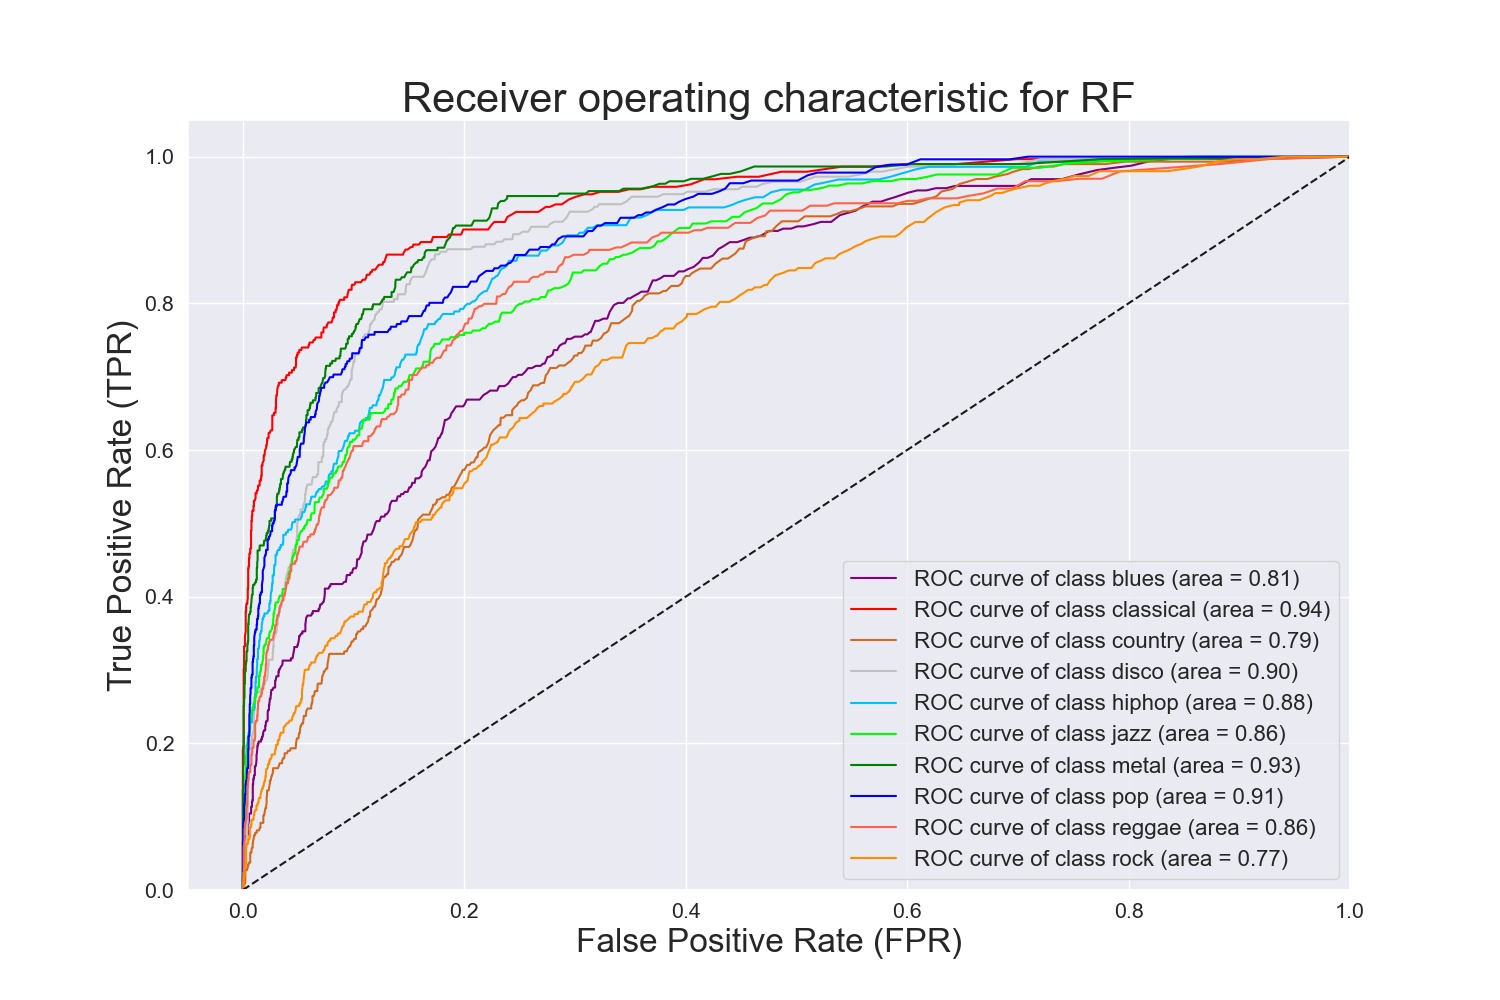
\includegraphics[width=\textwidth]{plot/SL/time_features/RF_10000_10GEN_GTZAN - ROC Plot.jpg}
            \caption{RF Time Features}
            \label{fig:RF Time Features}
        \end{minipage}
        \begin{minipage}[t]{.24\textwidth}
            \centering
            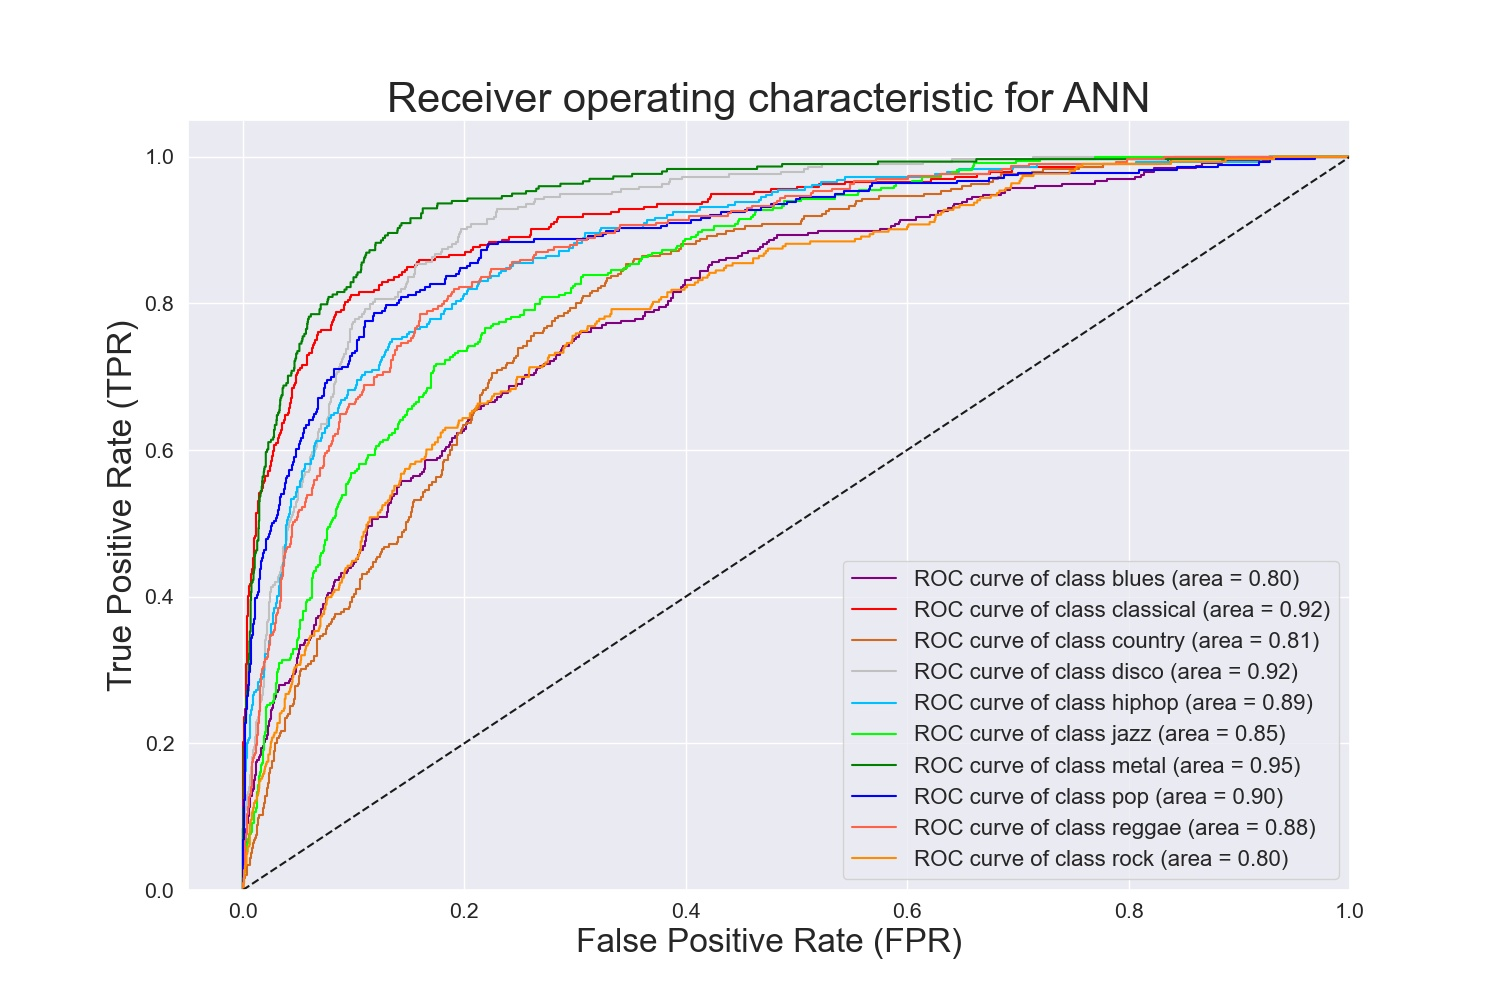
\includegraphics[width=\textwidth]{plot/SL/time_features/ANN_10000_10GEN_GTZAN - ROC Plot.jpg}
            \caption{ANN Time Features}
            \label{fig:ANN Time Features}
        \end{minipage}
        \begin{minipage}[t]{.24\textwidth}
            \centering
            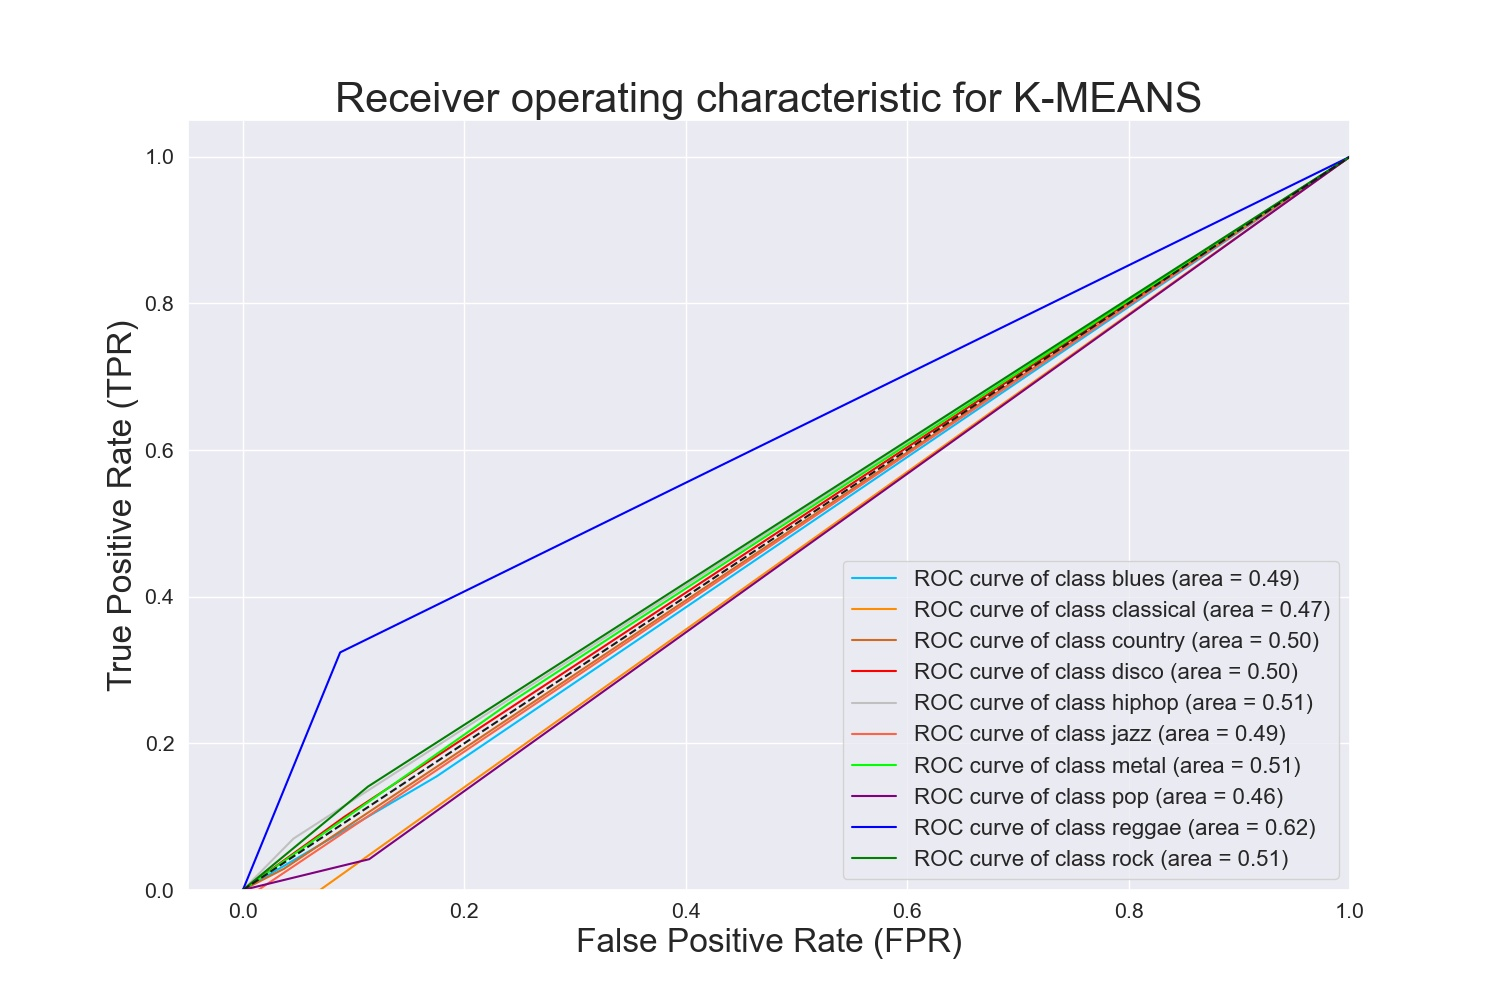
\includegraphics[width=\textwidth]{plot/UL/time_features/10000_10GEN_GTZAN - ROC Plot.jpg}
            \caption{K-Means Time Features}
            \label{fig:K-Means Time Features}
        \end{minipage}
    \end{center}
\end{figure}

\noindent
Using this type of features and the large number of clusters, it's possible to notice from Fig. \ref{fig:K-Means Time Features} that the k-means algorithm isn't very performing given the high data density and the non-globular shapes, the supervised algorithms behave much better. With reference to the number of clusters, it's possible to verify and evaluate the most appropriate value using the Silhouette algorithm. The second series of graphs involves the second set of features, that is the frequency domain features. In this evaluation we were able to evaluate the impact of the number of mel-frequency cepstrum coefficients.

\begin{figure}[!ht]
    \begin{center}
        \small\textbf{13 MFFCs - ROC results curves for frequency features extractions}\par\medskip    
        \begin{minipage}[t]{.24\textwidth}
            \centering
            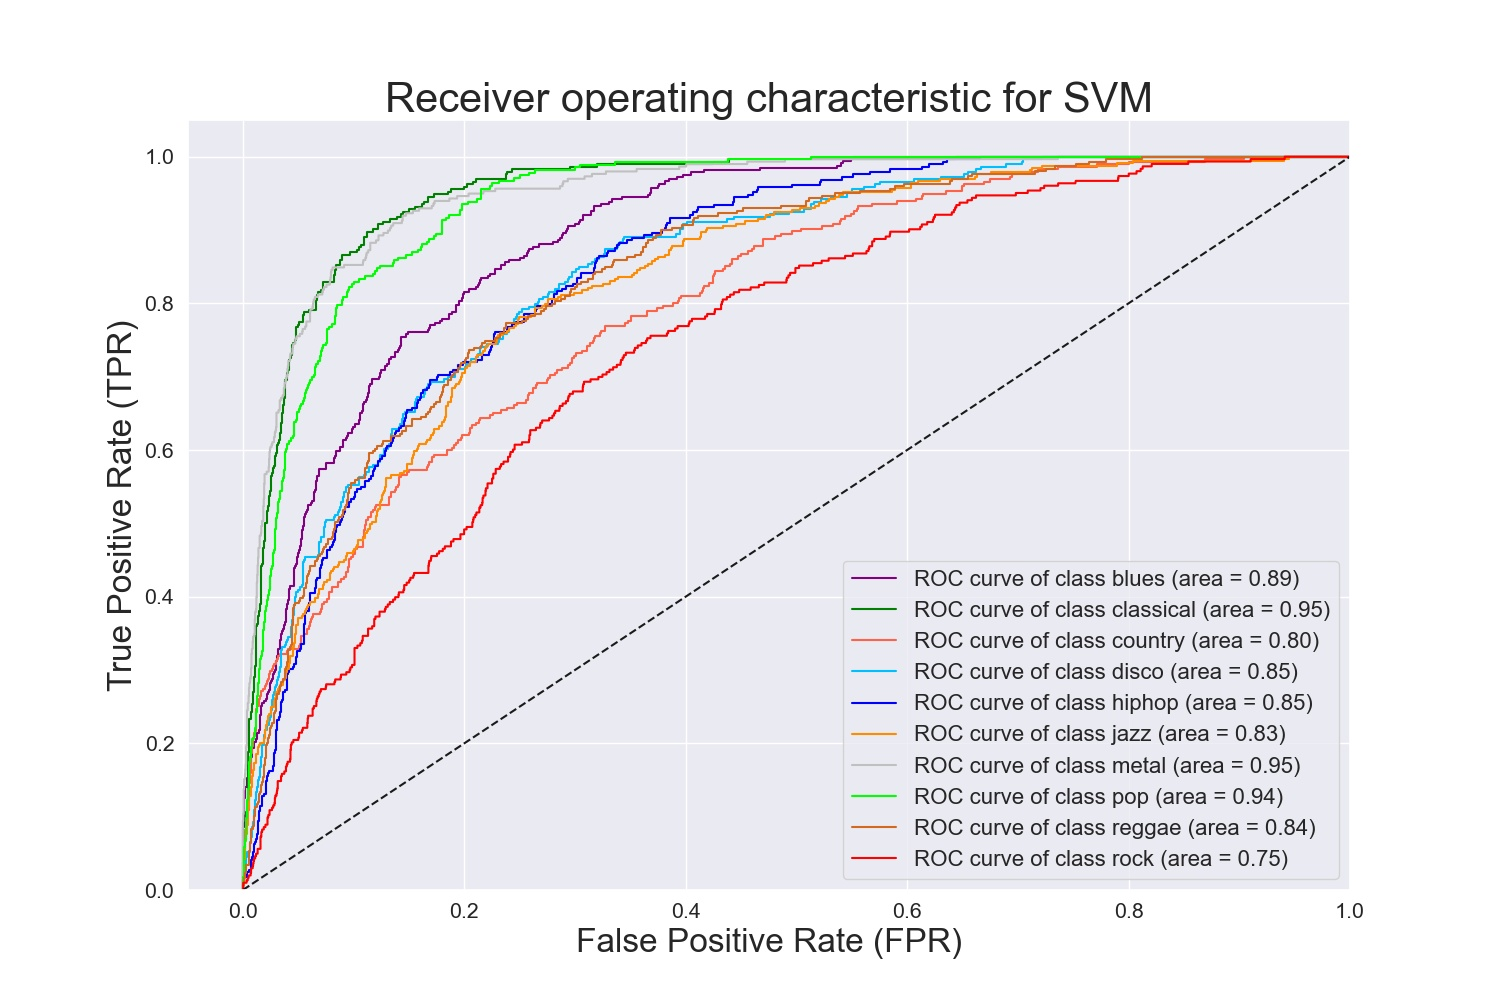
\includegraphics[width=\textwidth]{plot/SL/frequency_features/13/SVM_13MFCC_10000_10GEN_GTZAN - ROC Plot.jpg}
            \caption{13MFCCs SVM}
            \label{fig:13MFCCs SVM Frequency Features}
        \end{minipage}
        \begin{minipage}[t]{.24\textwidth}
            \centering
            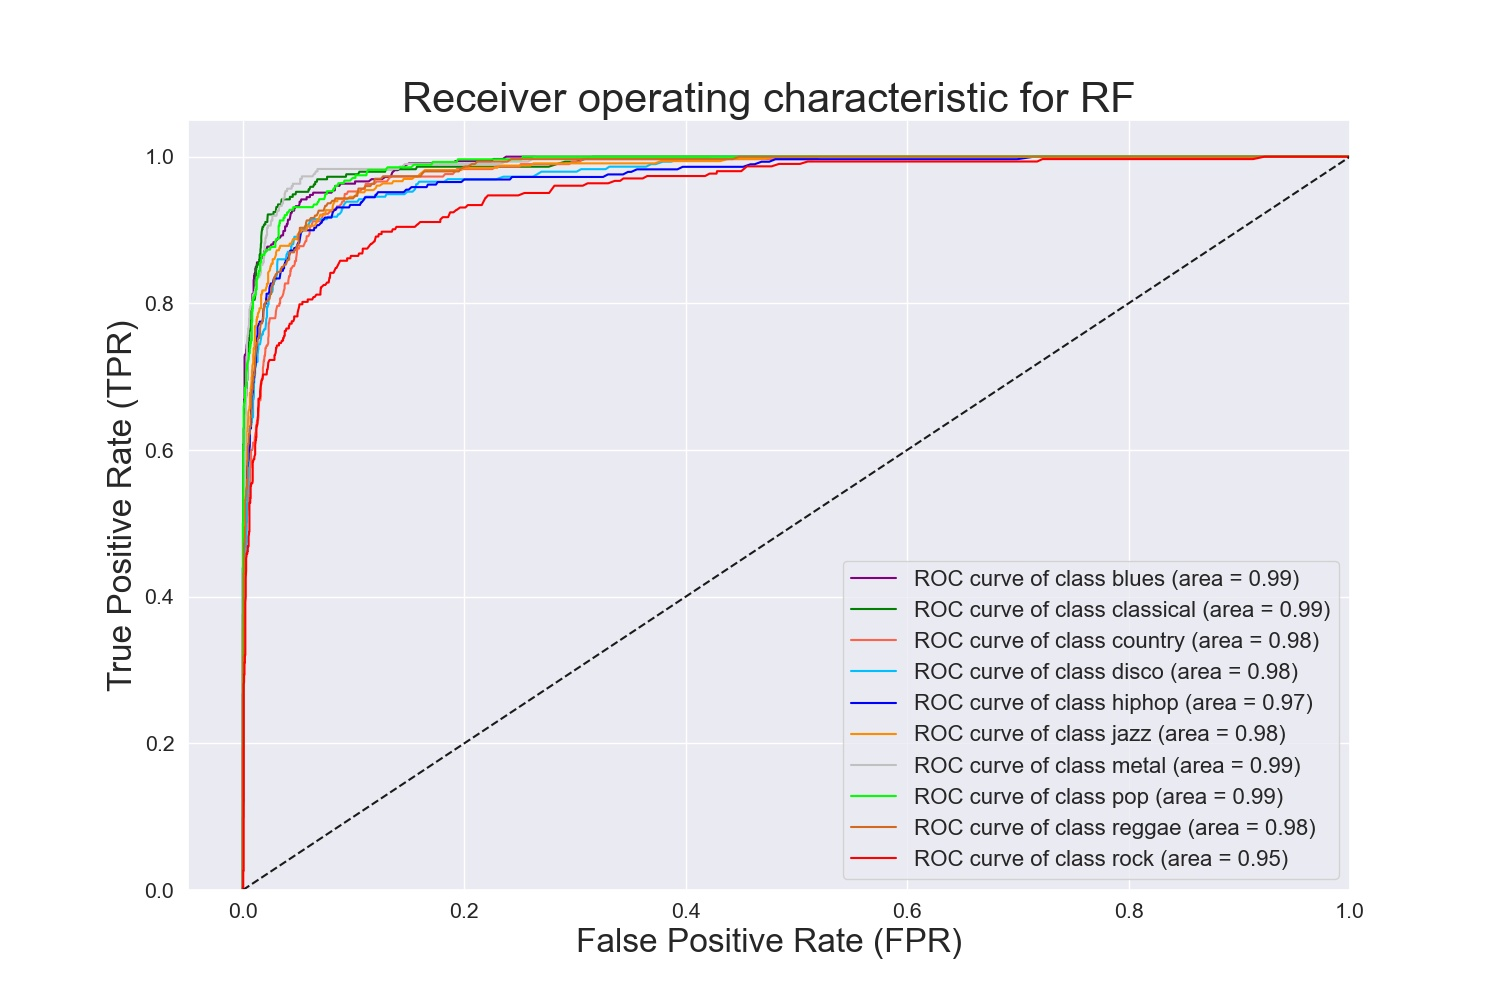
\includegraphics[width=\textwidth]{plot/SL/frequency_features/13/RF_13MFCC_10000_10GEN_GTZAN - ROC Plot.jpg}
            \caption{13MFCCs RF}
            \label{fig:13MFCCs RF Frequency Features}
        \end{minipage}
        \begin{minipage}[t]{.24\textwidth}
            \centering
            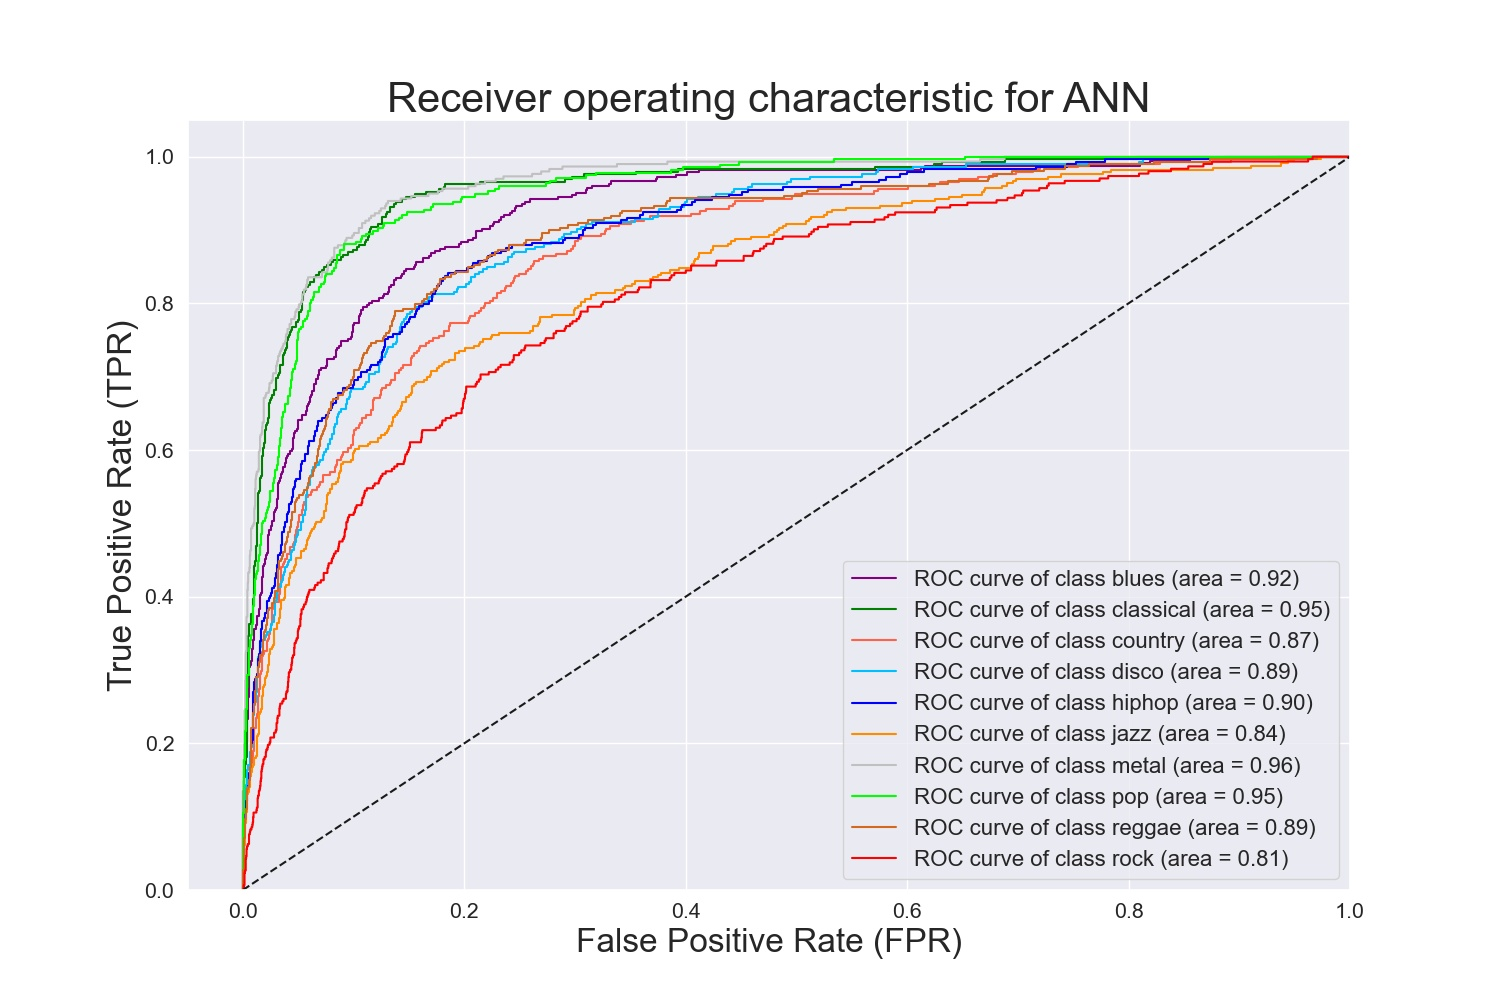
\includegraphics[width=\textwidth]{plot/SL/frequency_features/13/ANN_13MFCC_10000_10GEN_GTZAN - ROC Plot.jpg}
            \caption{13MFCCs ANN}
            \label{fig:13MFCCs ANN Frequency Features}
        \end{minipage}
        \begin{minipage}[t]{.24\textwidth}
            \centering
            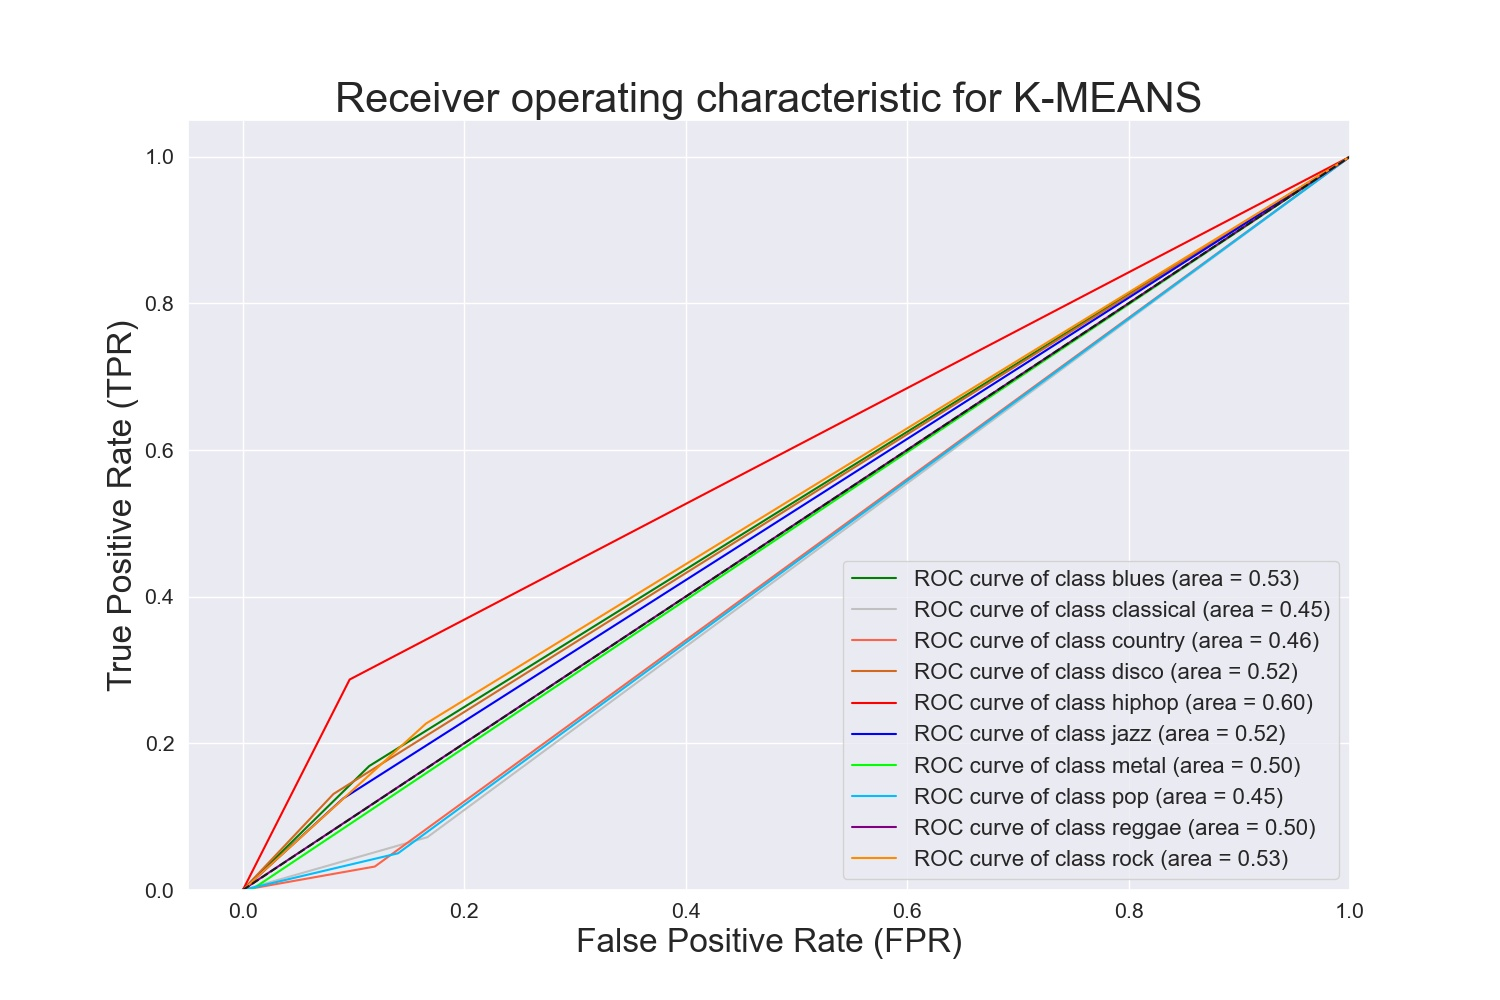
\includegraphics[width=\textwidth]{plot/UL/frequency_features/13/13MFCC_10000_10GEN_GTZAN - ROC Plot.jpg}
            \caption{13MFCCs K-Means}
            \label{fig:13MFCCs K-Means Frequency Features}
        \end{minipage}
    \end{center}
\end{figure}

\begin{table}[!ht]
    \centering
    \caption{13MFCCs supervised approach frequency features}
    \label{tab:13MFCCs Frequency Features Table Results}
    \begin{tabular}{c c c c c}
    \toprule
    &\multicolumn{4}{c}{13MFCCs}\\
    \cmidrule{2-5}
        Classifier  &Acc(\%) &RMSE &F1 &Ex.Time(s)\\
    \midrule 
        SVM             &49,60  &2,94 &0,48 &43,62\\    
        RF              &\textbf{81,56}&\textbf{1,85}&\textbf{0,81}&\textbf{52,98}\\
        ANN             &56,69  &2,77 &0,56 &519,50\\
    \bottomrule
    \end{tabular}
\end{table} 

\begin{figure}[!ht]
    \begin{center}
        \small\textbf{20 MFFCs - ROC results curves for frequency features}\par\medskip    
        \begin{minipage}[t]{.24\textwidth}
            \centering
            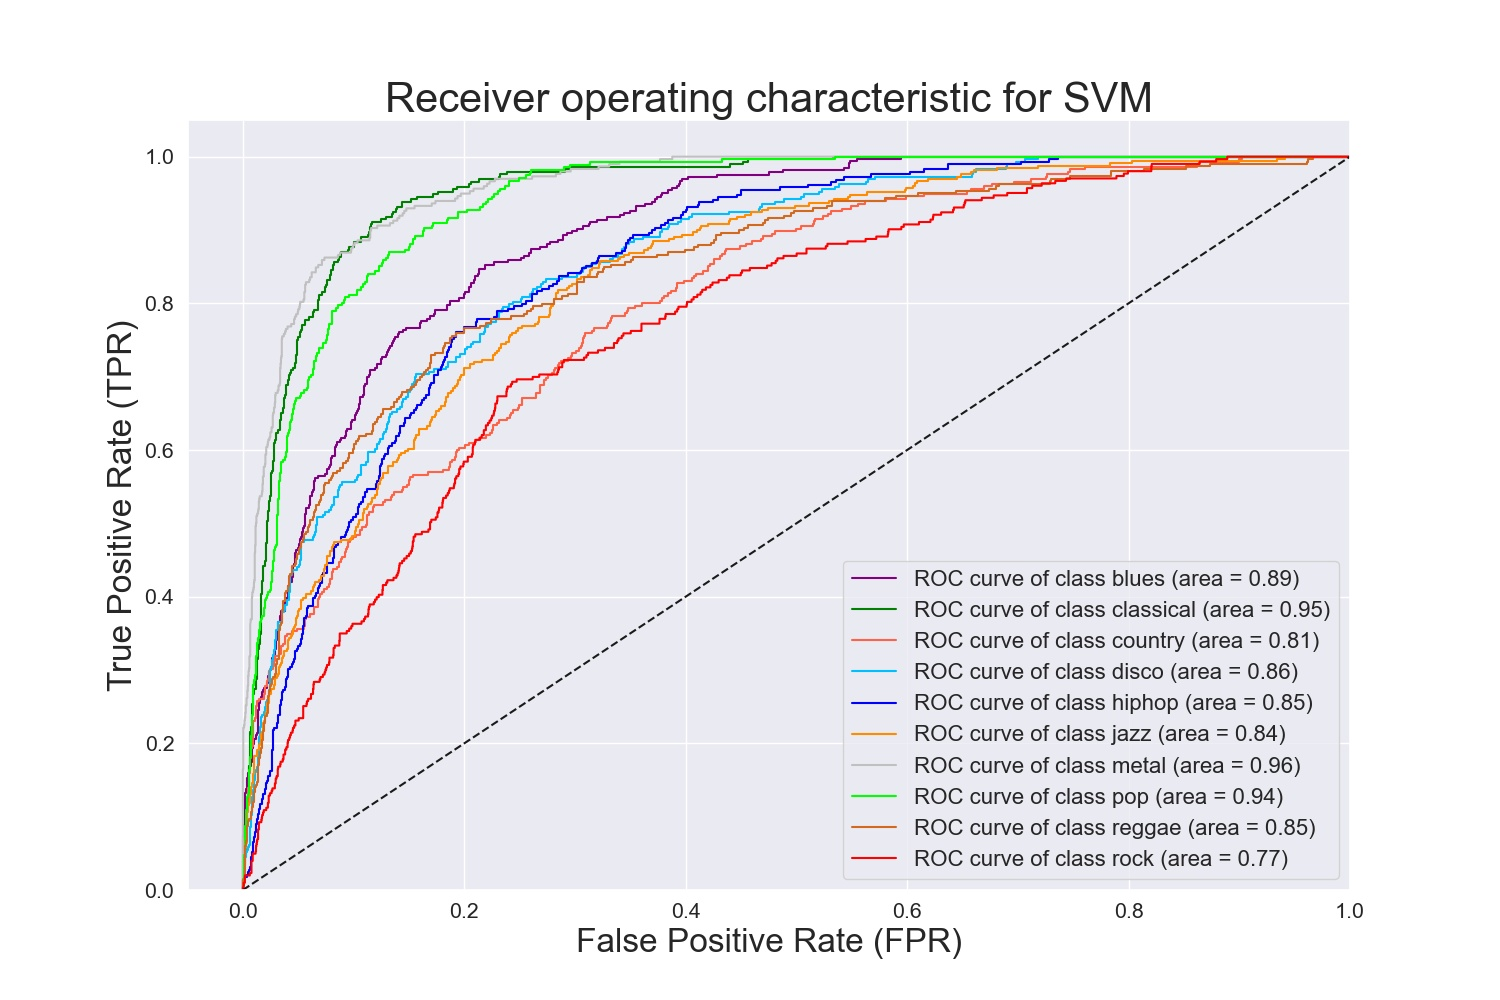
\includegraphics[width=\textwidth]{plot/SL/frequency_features/20/SVM_20MFCC_10000_10GEN_GTZAN - ROC Plot.jpg}
            \caption{20MFCCs SVM}
            \label{fig:20MFCCs SVM Frequency Features}
        \end{minipage}
        \begin{minipage}[t]{.24\textwidth}
            \centering
            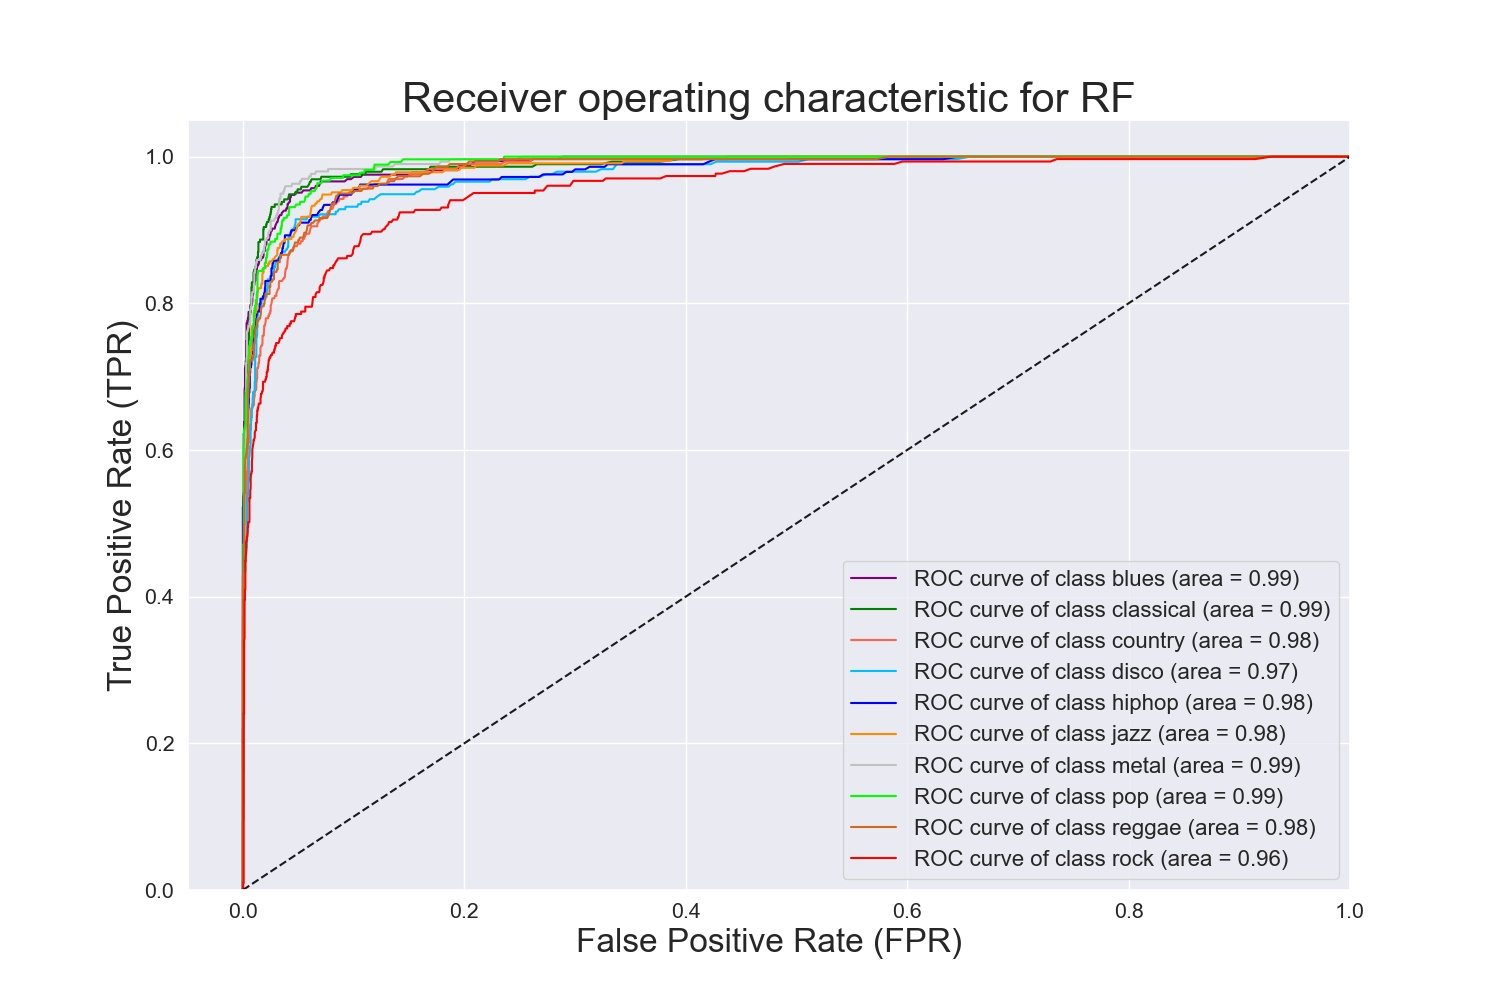
\includegraphics[width=\textwidth]{plot/SL/frequency_features/20/RF_20MFCC_10000_10GEN_GTZAN - ROC Plot.jpg}
            \caption{20MFCCs RF}
            \label{fig:20MFCCs RF Frequency Features}
        \end{minipage}
        \begin{minipage}[t]{.24\textwidth}
            \centering
            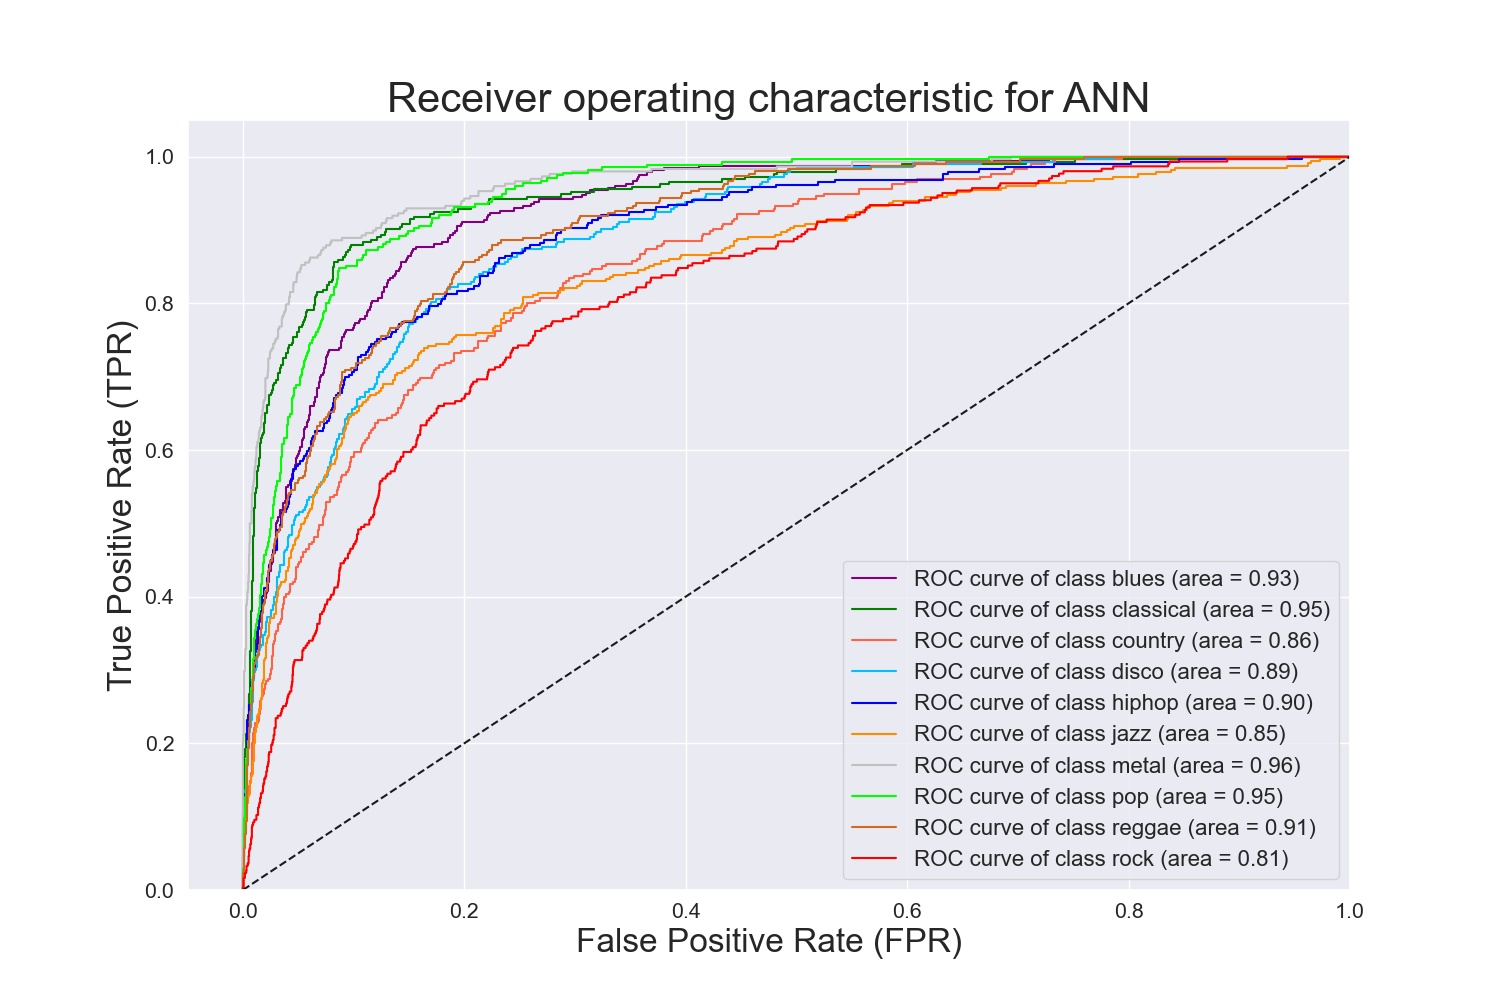
\includegraphics[width=\textwidth]{plot/SL/frequency_features/20/ANN_20MFCC_10000_10GEN_GTZAN - ROC Plot.jpg}
            \caption{20MFCCs ANN}
            \label{fig:20MFCCs ANN Frequency Features}
        \end{minipage}
        \begin{minipage}[t]{.24\textwidth}
            \centering
            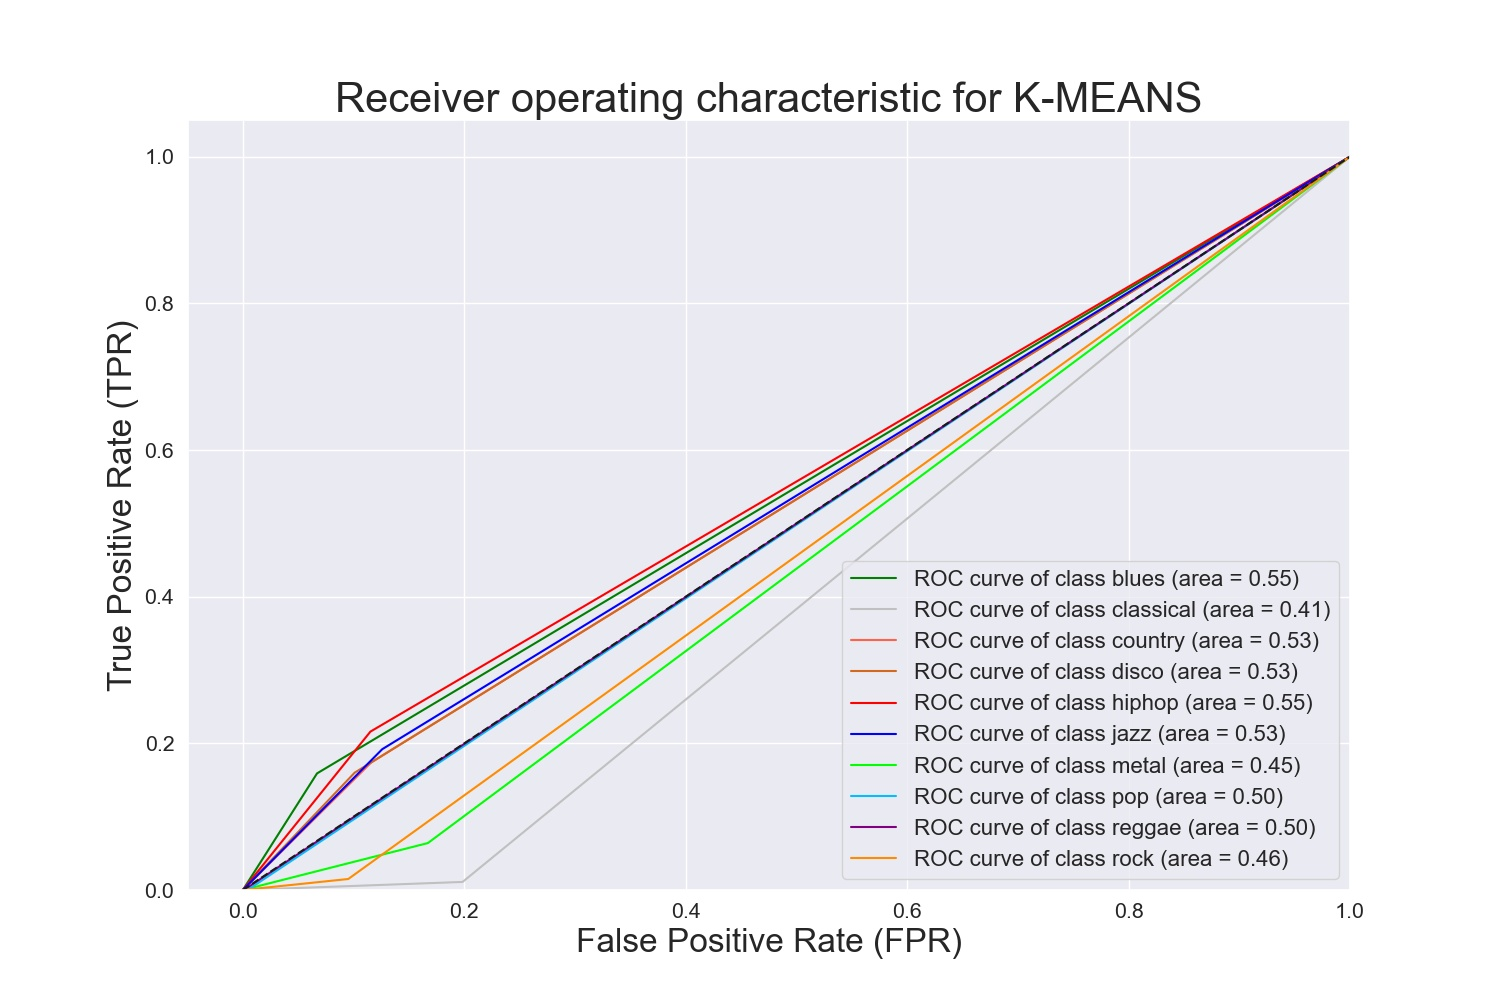
\includegraphics[width=\textwidth]{plot/UL/frequency_features/20/20MFCC_10000_10GEN_GTZAN - ROC Plot.jpg}
            \caption{20MFCCs K-Means}
            \label{fig:20MFCCs K-Means Frequency Features}
        \end{minipage}
    \end{center}
\end{figure}

\begin{table}[!ht]
    \centering
    \caption{20MFCCs supervised approach frequency features}
    \label{tab:20MFCCs Frequency Features Table Results}
    \begin{tabular}{c c c c c}
    \toprule
    &\multicolumn{4}{c}{20MFCCs}\\
    \cmidrule{2-5}
        Classifier  &Acc(\%) &RMSE &F1 &Ex.Time(s)\\
    \midrule 
        SVM             &50,96 &2,90 &0,49  &45,84\\    
        RF              &\textbf{82,39}&\textbf{1,76}&\textbf{0,82}&\textbf{55,34}\\
        ANN             &56,39 &2,74 &0,56  &499,91\\
    \bottomrule
    \end{tabular}
\end{table}

\begin{figure}[!ht]
    \begin{center}
        \small\textbf{40 MFFCs - ROC results curves for frequency features}\par\medskip    
        \begin{minipage}[t]{.24\textwidth}
            \centering
            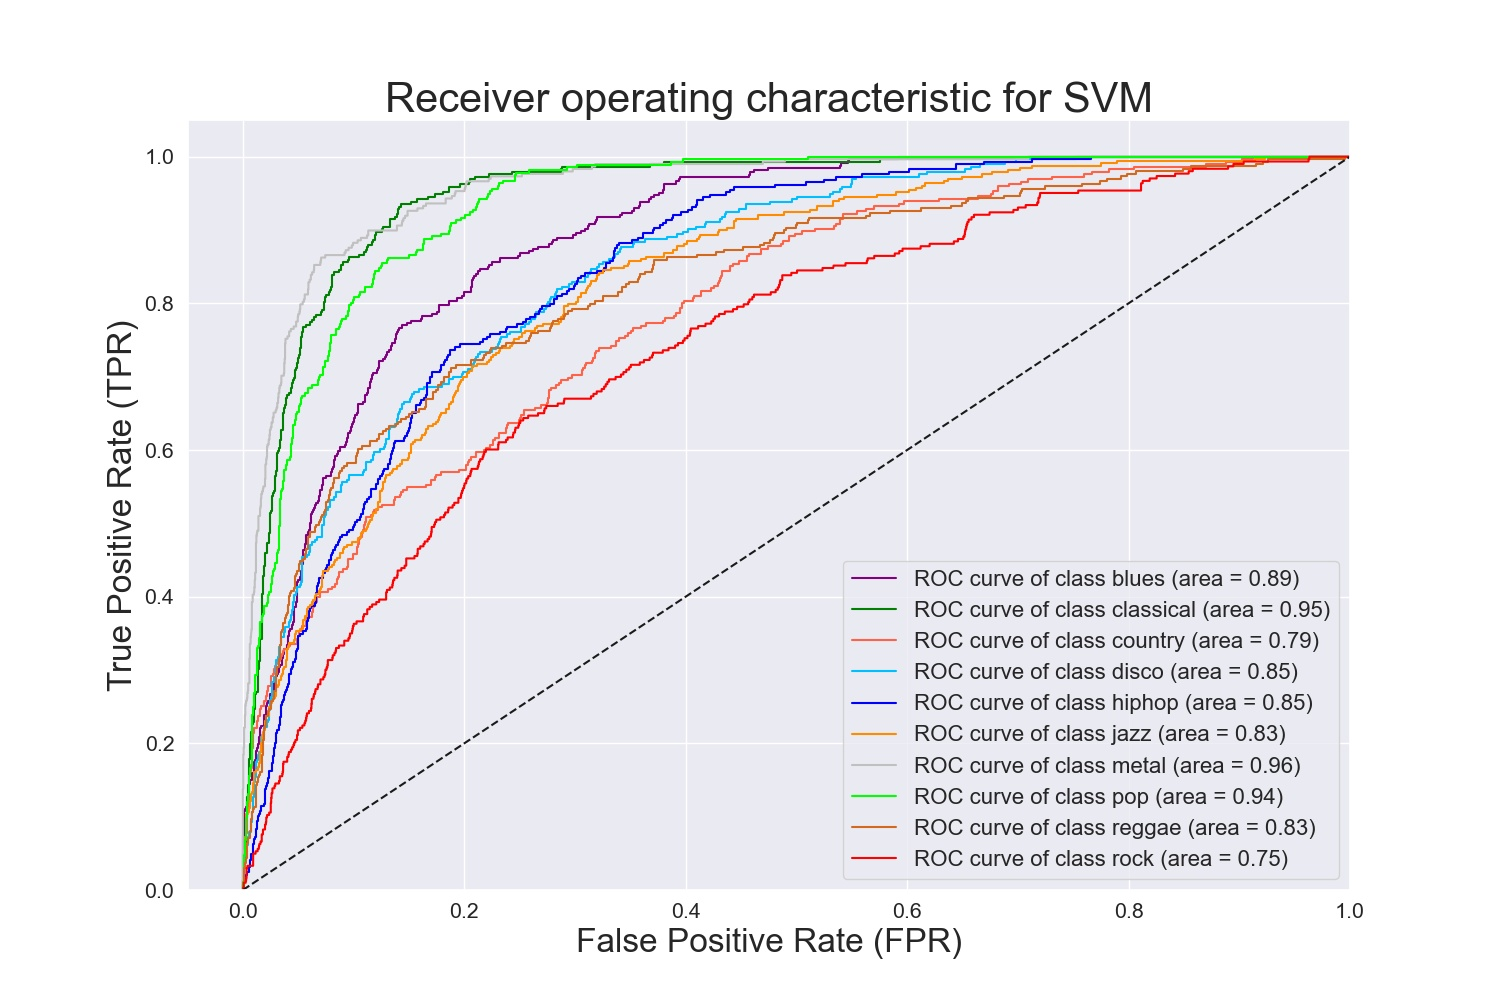
\includegraphics[width=\textwidth]{plot/SL/frequency_features/40/SVM_40MFCC_10000_10GEN_GTZAN - ROC Plot.jpg}
            \caption{40MFCCs SVM}
            \label{fig:40MFCCs SVM Frequency Features}
        \end{minipage}
        \begin{minipage}[t]{.24\textwidth}
            \centering
            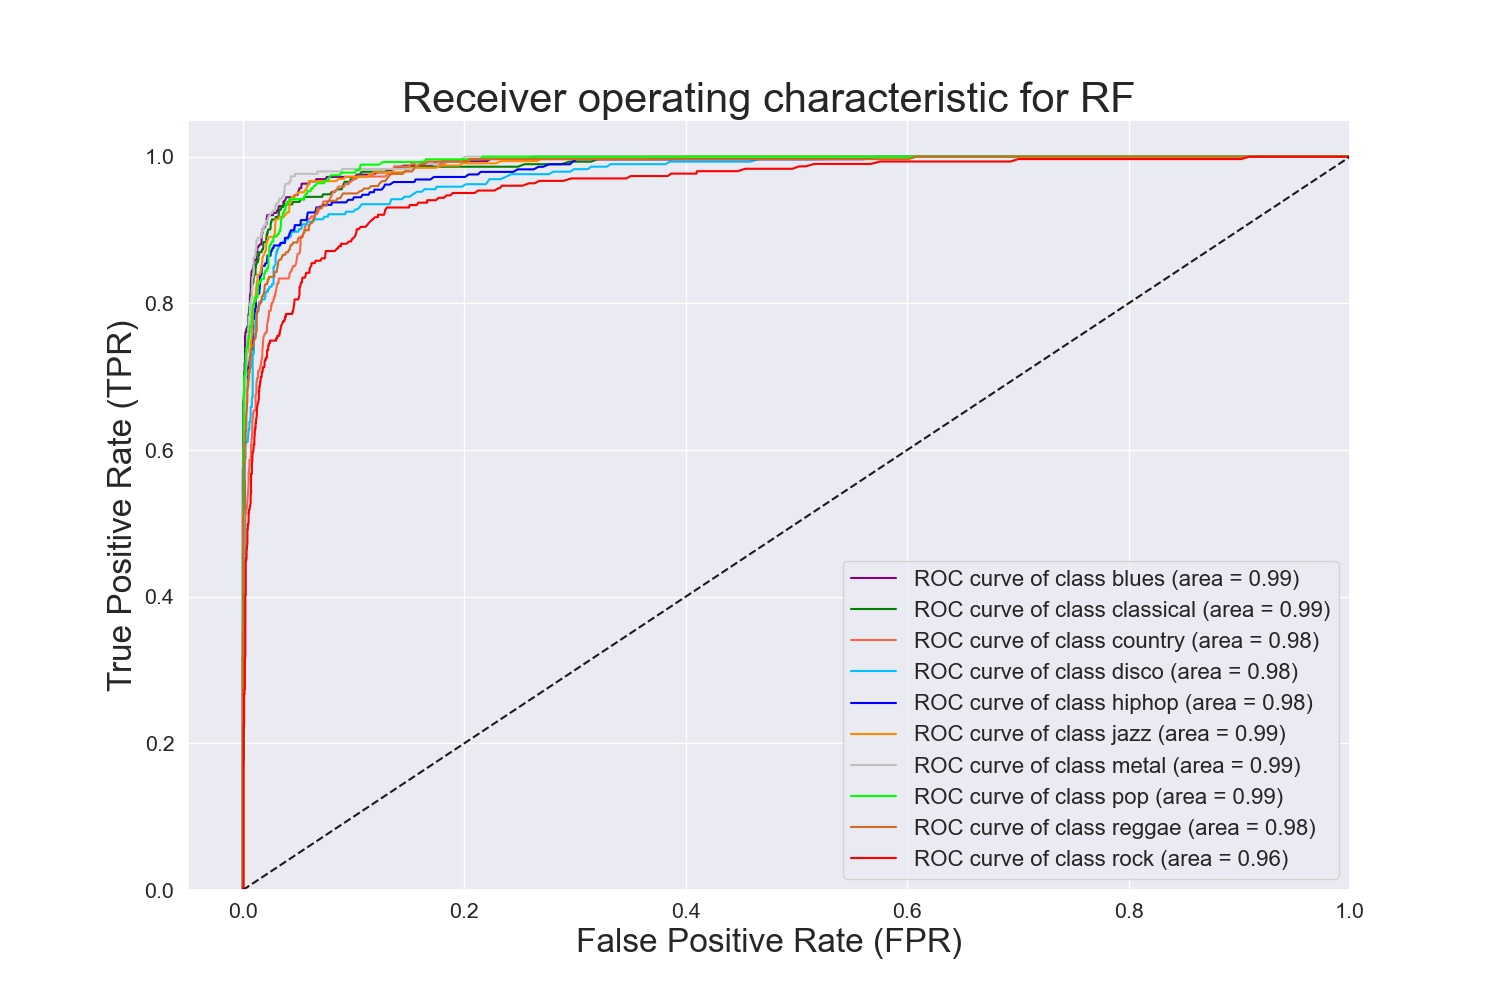
\includegraphics[width=\textwidth]{plot/SL/frequency_features/40/RF_40MFCC_10000_10GEN_GTZAN - ROC Plot.jpg}
            \caption{40MFCCs RF}
            \label{fig:40MFCCs RF Frequency Features}
        \end{minipage}
        \begin{minipage}[t]{.24\textwidth}
            \centering
            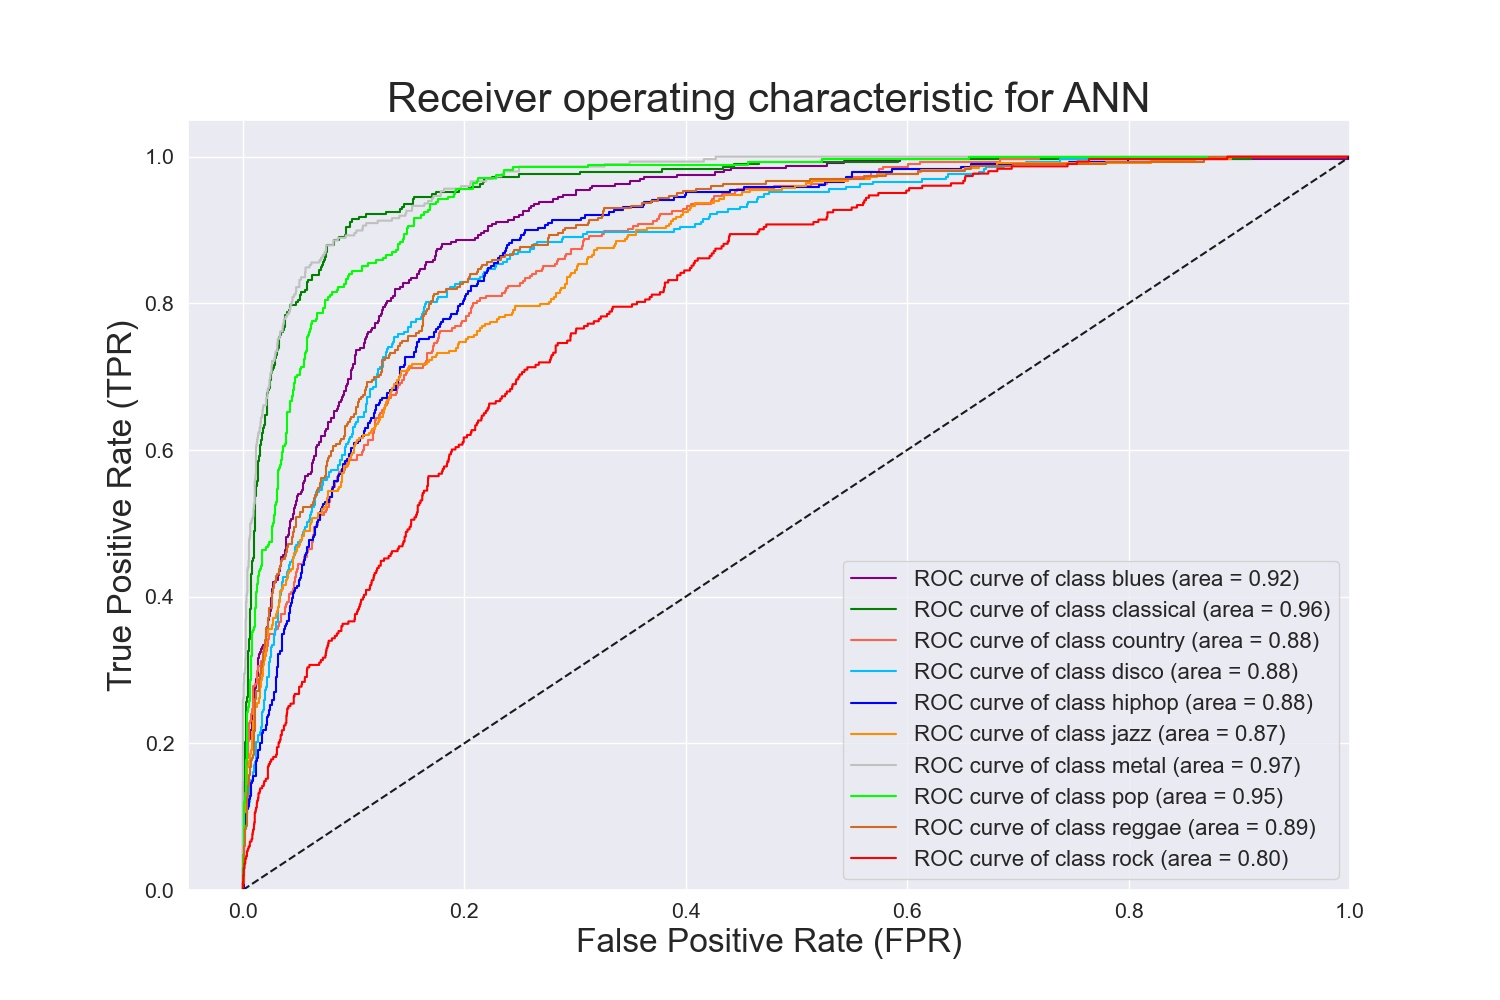
\includegraphics[width=\textwidth]{plot/SL/frequency_features/40/ANN_40MFCC_10000_10GEN_GTZAN - ROC Plot.jpg}
            \caption{40MFCCs ANN}
            \label{fig:40MFCCs ANN Frequency Features}
        \end{minipage}
        \begin{minipage}[t]{.24\textwidth}
            \centering
            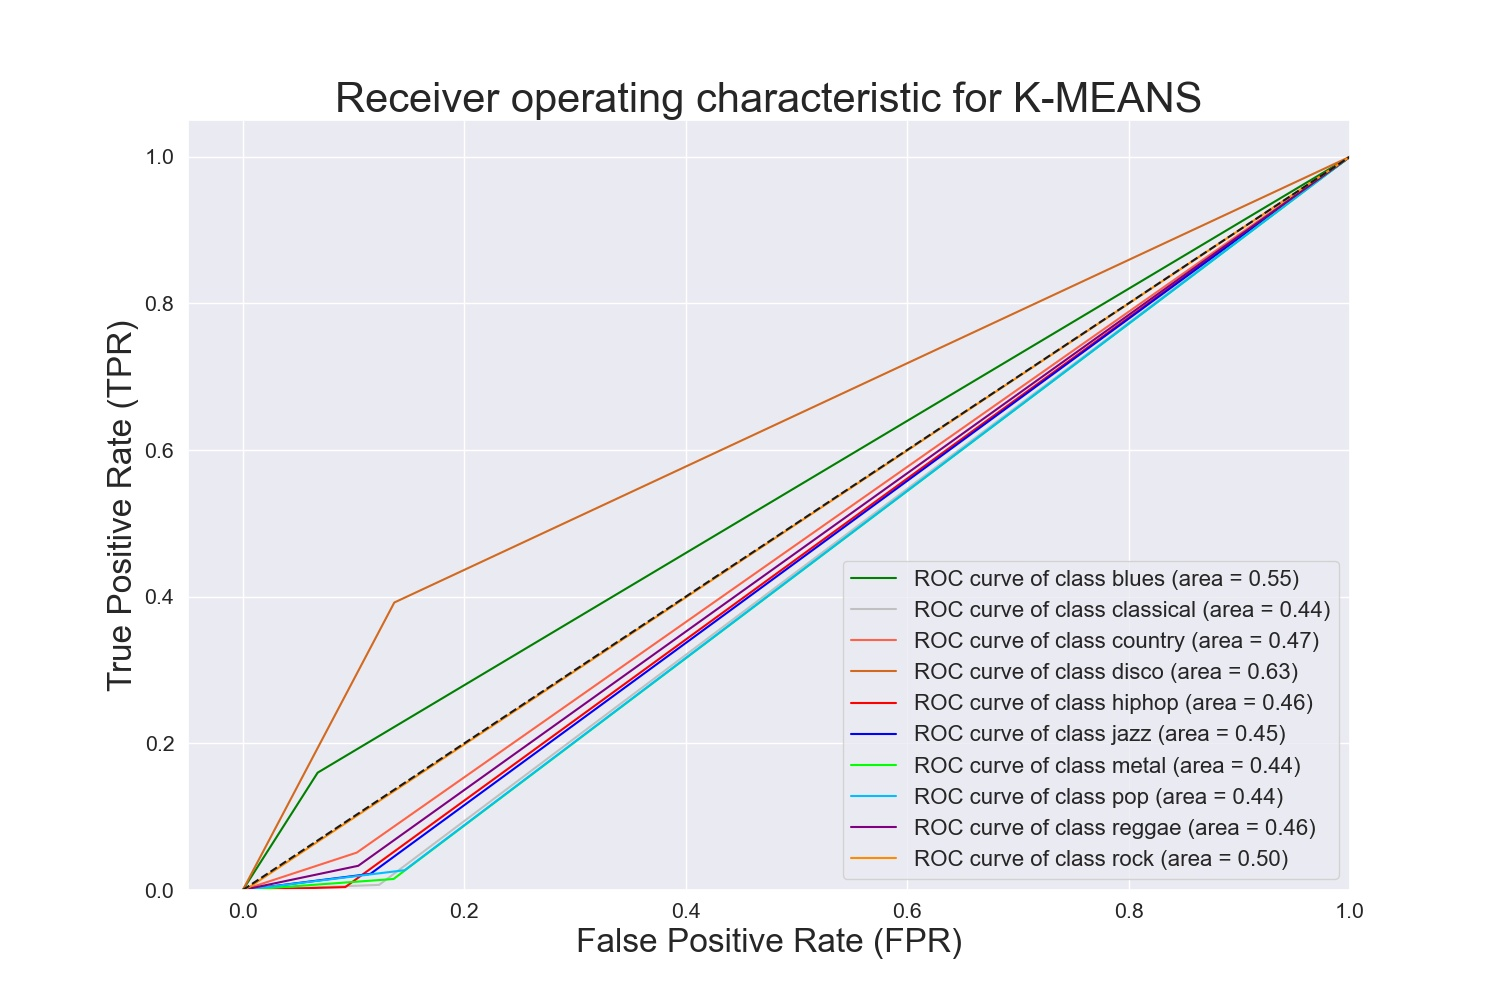
\includegraphics[width=\textwidth]{plot/UL/frequency_features/40/40MFCC_10000_10GEN_GTZAN - ROC Plot.jpg}
            \caption{40MFCCs K-Means}
            \label{fig:40MFCCs K-Means Frequency Features}
        \end{minipage}
    \end{center}
\end{figure}

\begin{table}[!ht]
    \centering
    \caption{40MFCCs supervised approach frequency features}
    \label{tab:40MFCCs Frequency Features Table Results}
    \begin{tabular}{c c c c c}
    \toprule
    &\multicolumn{4}{c}{40MFCCs}\\
    \cmidrule{2-5}
        Classifier  &Acc(\%) &RMSE &F1 &Ex.Time(s)\\
    \midrule 
        SVM             &49,33 &2,97 &0,47  &49,79\\
        RF              &\textcolor{green}{\textbf{83,39}}&\textcolor{green}{\textbf{1,69}}
                        &\textcolor{green}{\textbf{0,83}}&\textcolor{green}{\textbf{65,04}}\\
        ANN             &52,76 &2,86 &0,52  &270,98\\
    \bottomrule
    \end{tabular}
\end{table}

\noindent
From data reported in Tables \ref{tab:13MFCCs Frequency Features Table Results}, \ref{tab:20MFCCs Frequency Features Table Results}, \ref{tab:40MFCCs Frequency Features Table Results} it's possible to verify how the increase of the spectral coefficients has led to a certain improvement. While as regards the classification of the K-Means algorithm by viewing the Figs. \ref{fig:13MFCCs K-Means Frequency Features}, \ref{fig:20MFCCs K-Means Frequency Features}, \ref{fig:40MFCCs K-Means Frequency Features}, it's possible to note that, even with a set of different and more explanatory features, it's performances are worse. It's also possible to note how for the different classifiers of the supervisioned approach, this features and the increase of the coefficients as a function of the execution time allows us to make detailed evaluations on which is the most suitable classifier for musical genres classification. You can see the best result among the three classifiers in bold, and the best among the three in green.

\newpage
\noindent
The last approach depicted is related to the fusion of the temporal and frequency features to verify the improvements obtained. 

\begin{figure}[!ht]
    \begin{center}
        \small\textbf{13 MFFCs - ROC results curves for Time+frequency features}\par\medskip
        \begin{minipage}[t]{.24\textwidth}
            \centering
            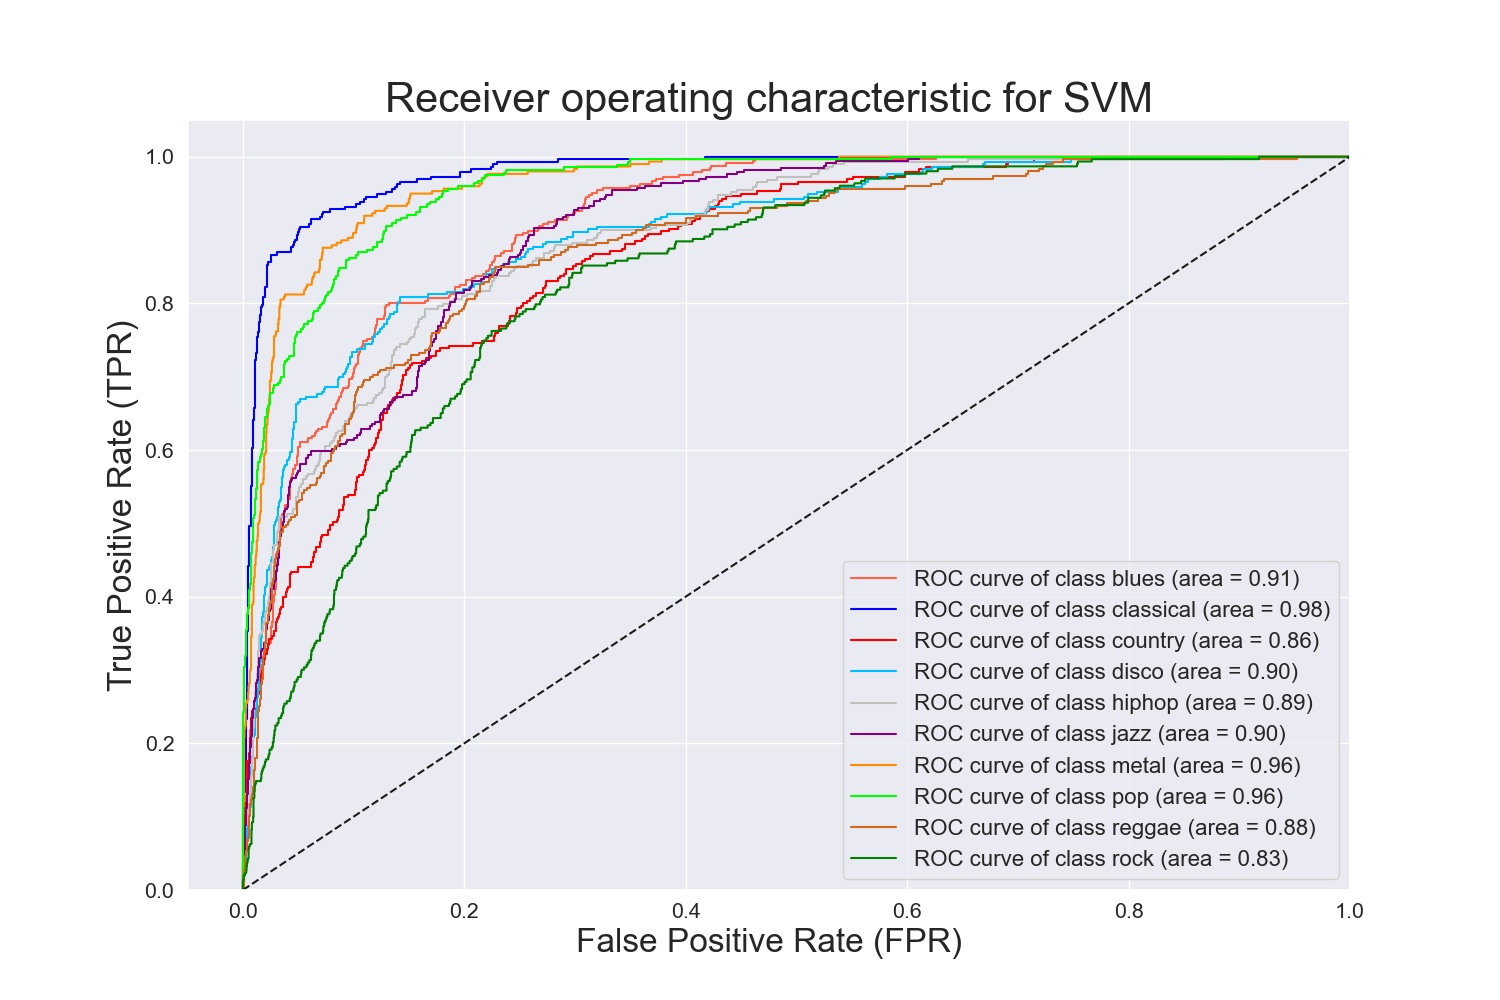
\includegraphics[width=\textwidth]{plot/SL/all_features/13/SVM_13MFCC_10000_10GEN_GTZAN - ROC Plot.jpg}
            \caption{13MFCCs SVM}
            \label{fig:13MFCCs SVM Time+frequency Features}
        \end{minipage}
        \begin{minipage}[t]{.24\textwidth}
            \centering
            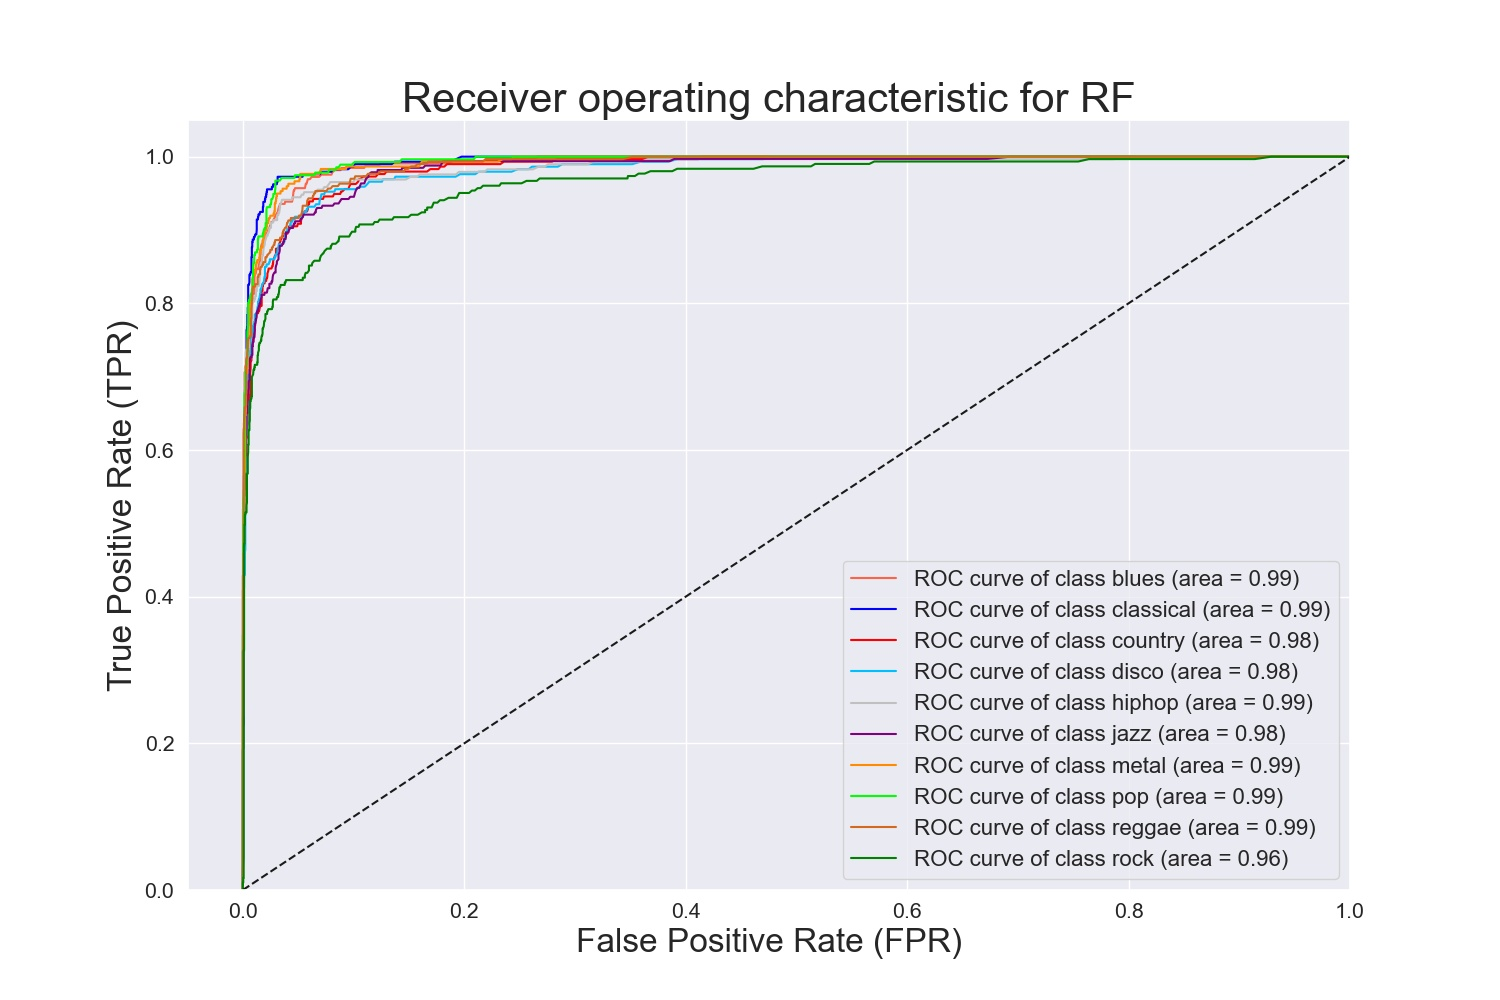
\includegraphics[width=\textwidth]{plot/SL/all_features/13/RF_13MFCC_10000_10GEN_GTZAN - ROC Plot.jpg}
            \caption{13MFCCs RF}
            \label{fig:13MFCCs RF Time+frequency Features}
        \end{minipage}
        \begin{minipage}[t]{.24\textwidth}
            \centering
            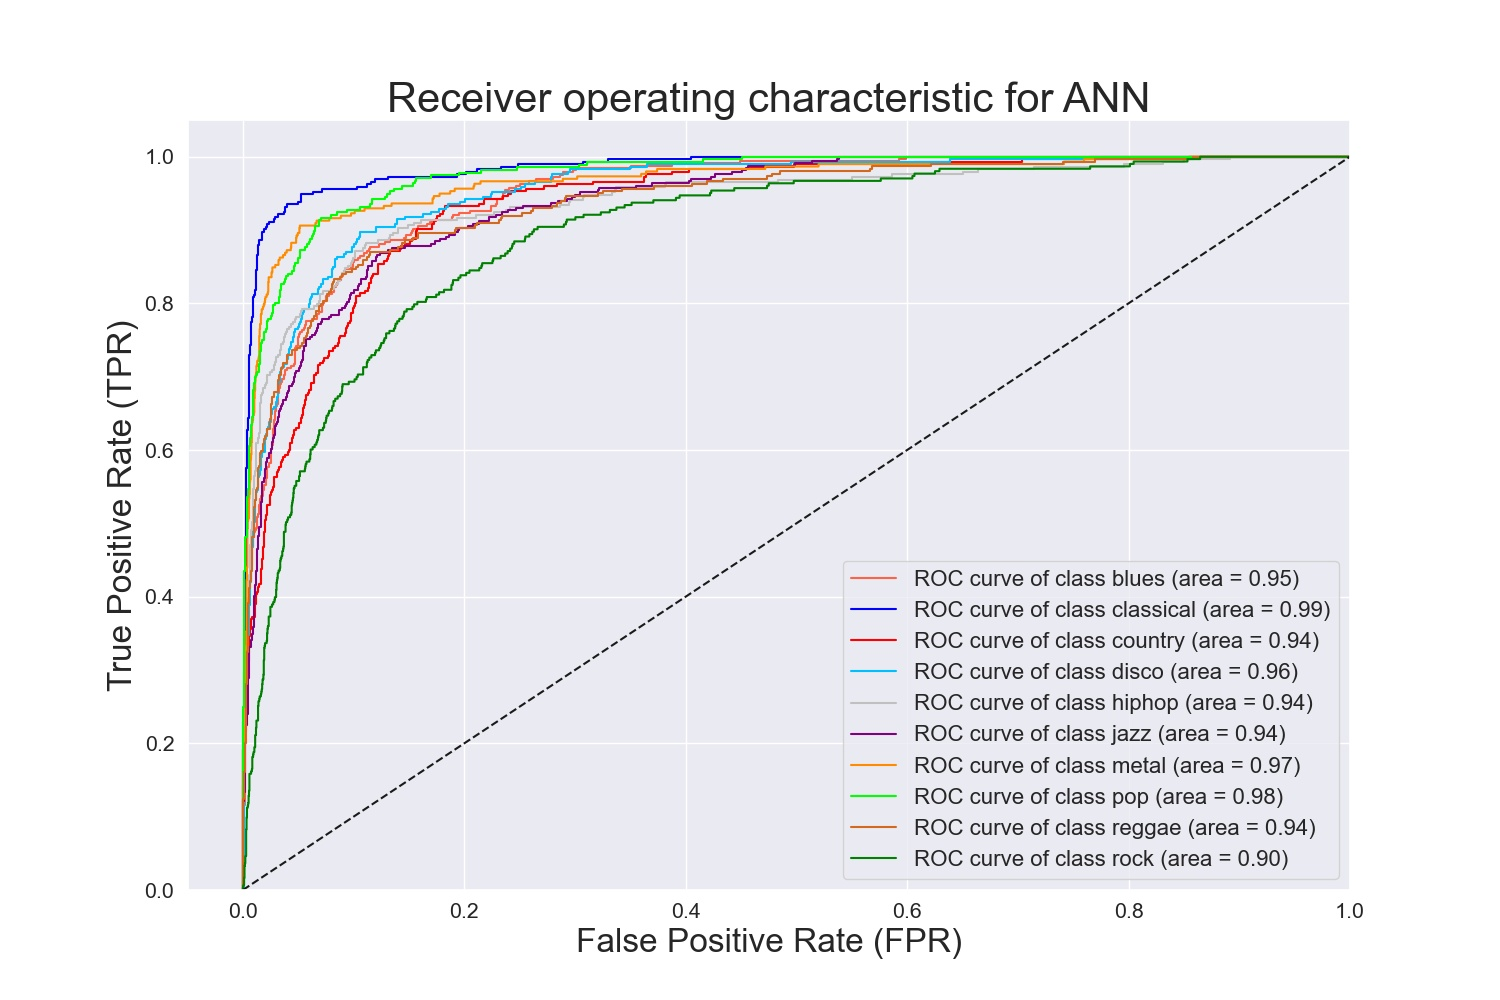
\includegraphics[width=\textwidth]{plot/SL/all_features/13/ANN_13MFCC_10000_10GEN_GTZAN - ROC Plot.jpg}
            \caption{13MFCCs ANN}
            \label{fig:13MFCCs ANN Time+frequency Features}
        \end{minipage}
        \begin{minipage}[t]{.24\textwidth}
            \centering
            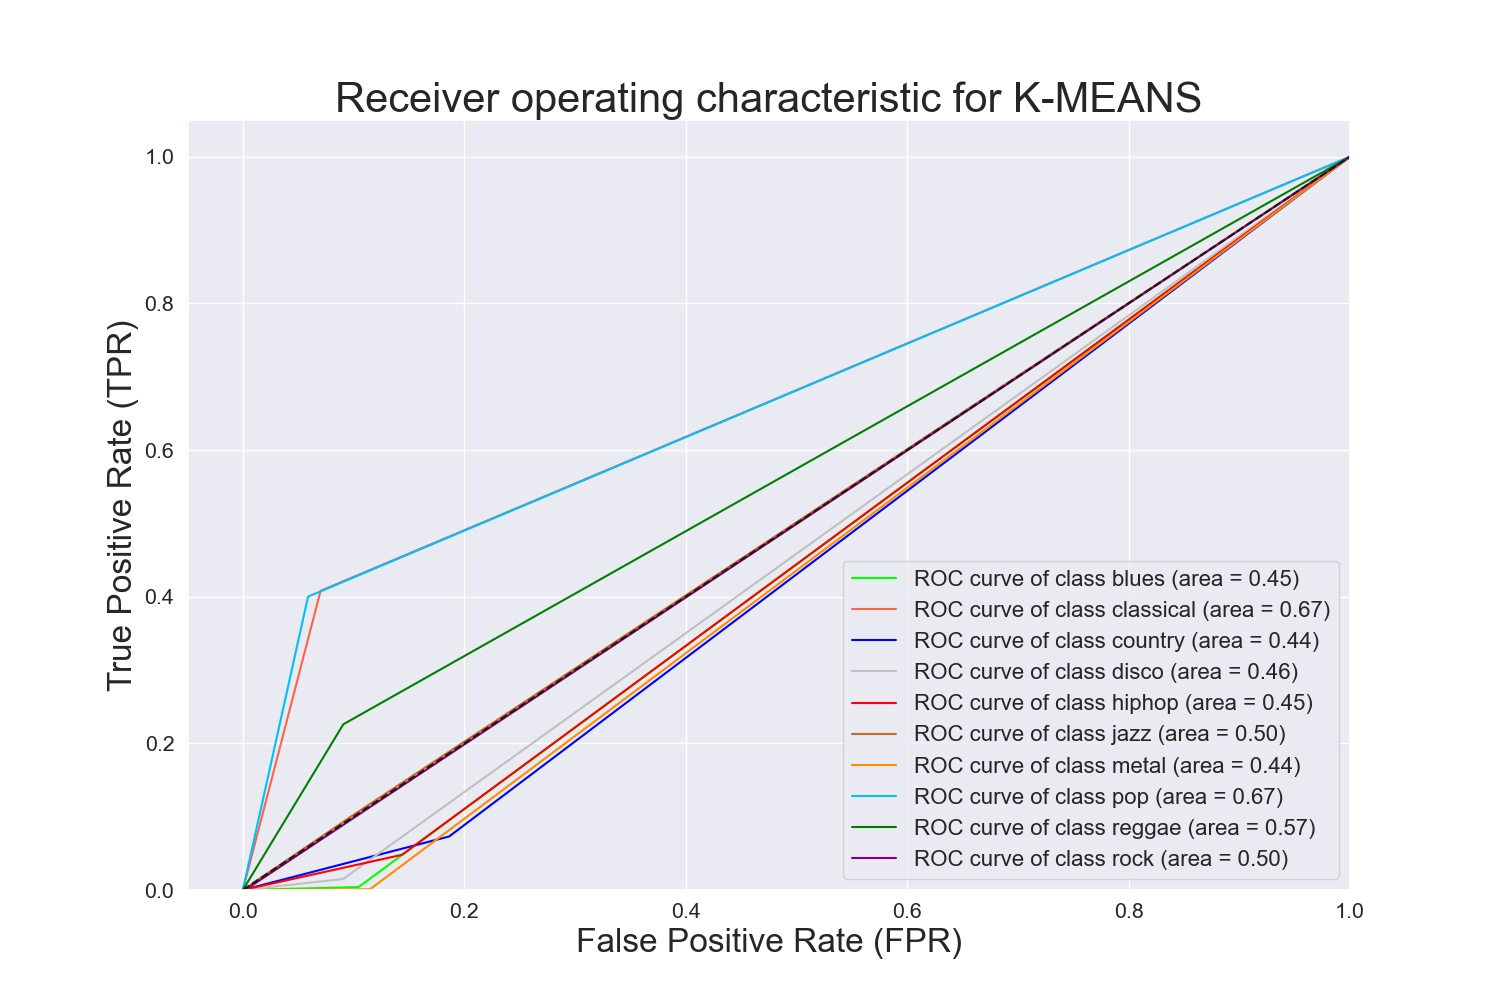
\includegraphics[width=\textwidth]{plot/UL/all_features/13/13MFCC_10000_10GEN_GTZAN - ROC Plot.jpg}
            \caption{13MFCCs K-Means}
            \label{fig:13MFCCs K-Means Time+frequency Features}
        \end{minipage}
    \end{center}
\end{figure}

\begin{table}[!ht]
    \centering
    \caption{13MFCCs supervised approach Time+frequency features}
    \label{tab:13MFCCs Time+Frequency Features Table Results}
    \begin{tabular}{c c c c c}
    \toprule
    &\multicolumn{4}{c}{13MFCCs}\\
    \cmidrule{2-5}
        Classifier  &Acc(\%) &RMSE &F1 &Ex.Time(s)\\
    \midrule 
        SVM             &60,09 &2,77 &0,59 &39,50\\
        RF              &\textbf{84,93}&\textbf{1,64}&\textbf{0,84}&\textbf{52,93}\\
        ANN             &70,06 &2,42 &0,70 &428,97\\
    \bottomrule
    \end{tabular}
\end{table}

\begin{figure}[!ht]
    \begin{center}
        \small\textbf{20 MFFCs - ROC results curves for Time+frequency features}\par\medskip
        \begin{minipage}[t]{.24\textwidth}
            \centering
            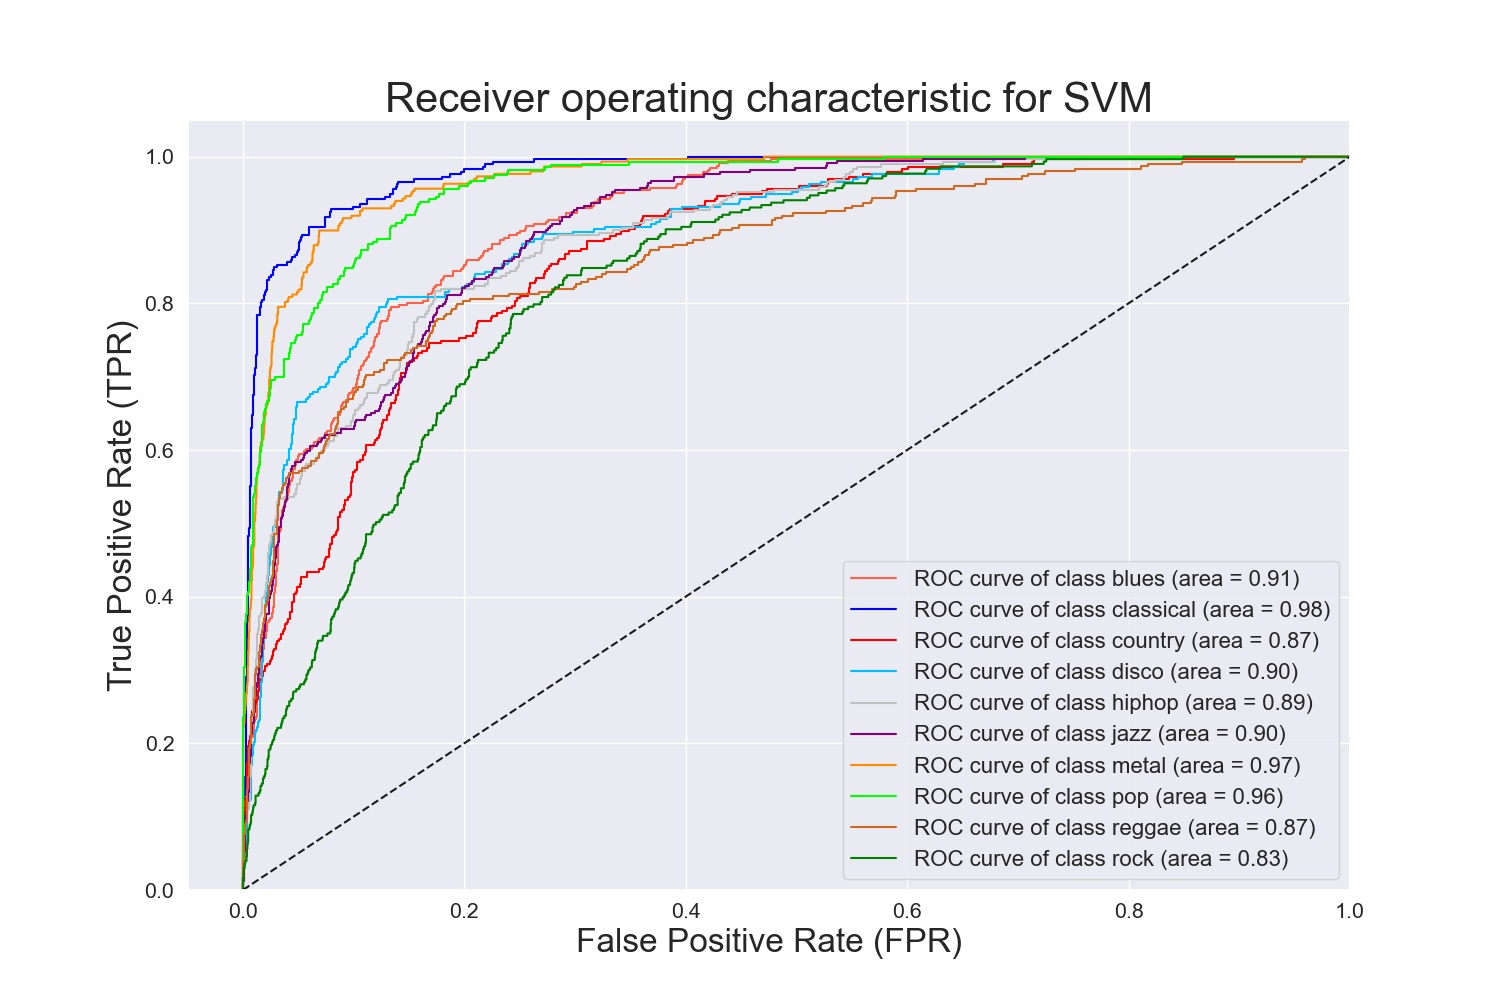
\includegraphics[width=\textwidth]{plot/SL/all_features/20/SVM_20MFCC_10000_10GEN_GTZAN - ROC Plot.jpg}
            \caption{20MFCCs SVM}
            \label{fig:20MFCCs SVM Time+frequency Features}
        \end{minipage}
        \begin{minipage}[t]{.24\textwidth}
            \centering
            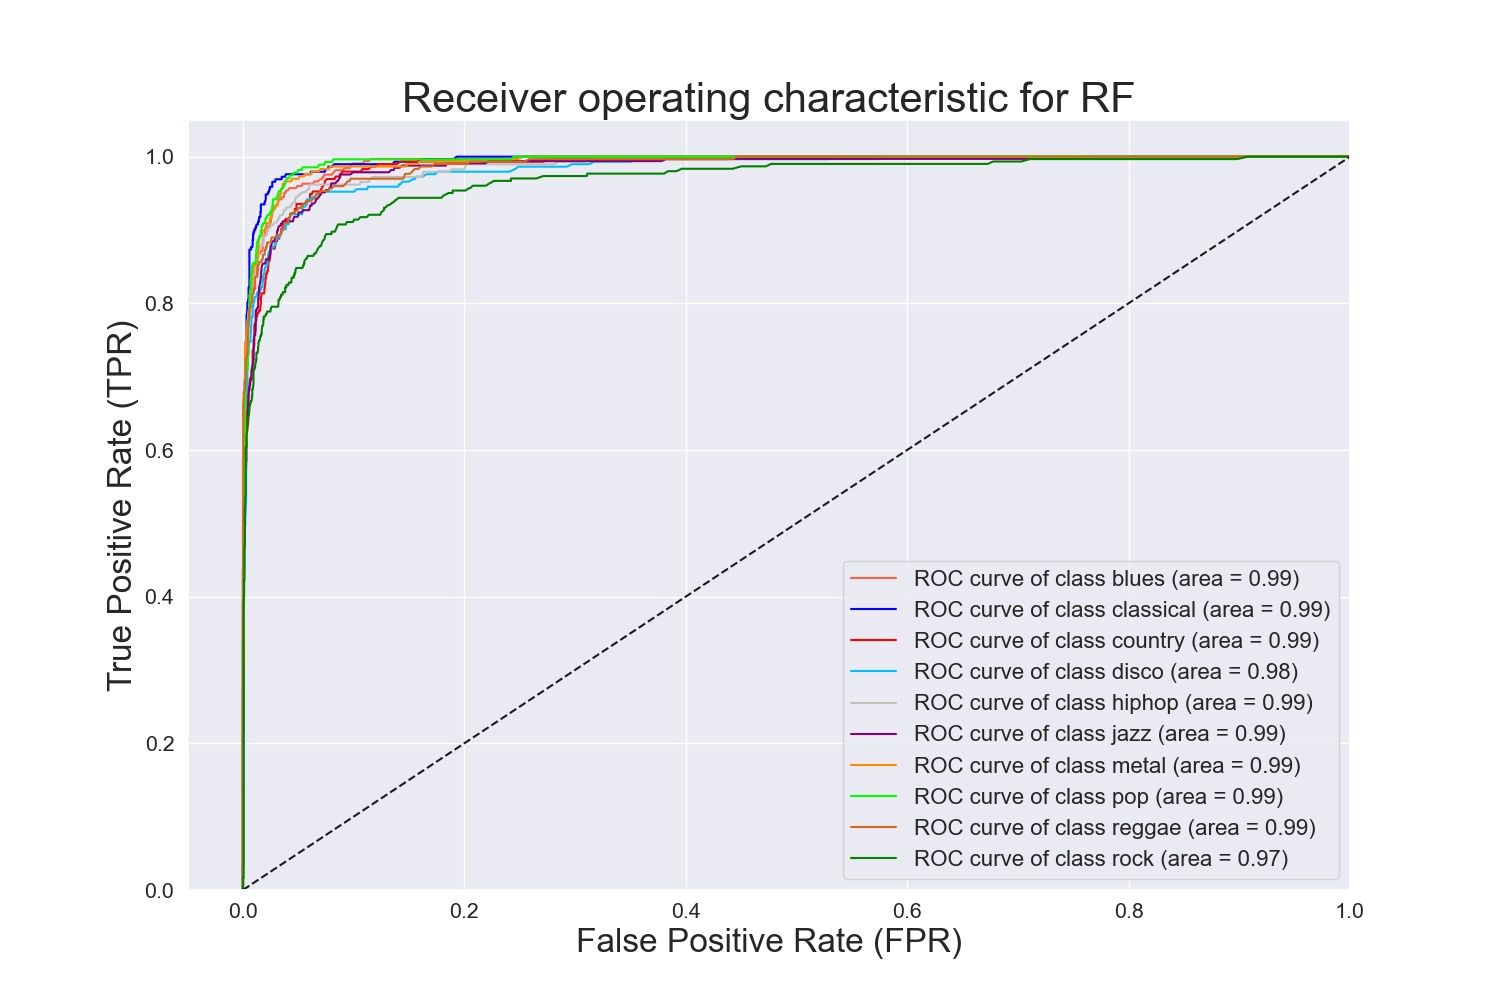
\includegraphics[width=\textwidth]{plot/SL/all_features/20/RF_20MFCC_10000_10GEN_GTZAN - ROC Plot.jpg}
            \caption{20MFCCs RF}
            \label{fig:20MFCCs RF Time+frequency Features}
        \end{minipage}
        \begin{minipage}[t]{.24\textwidth}
            \centering
            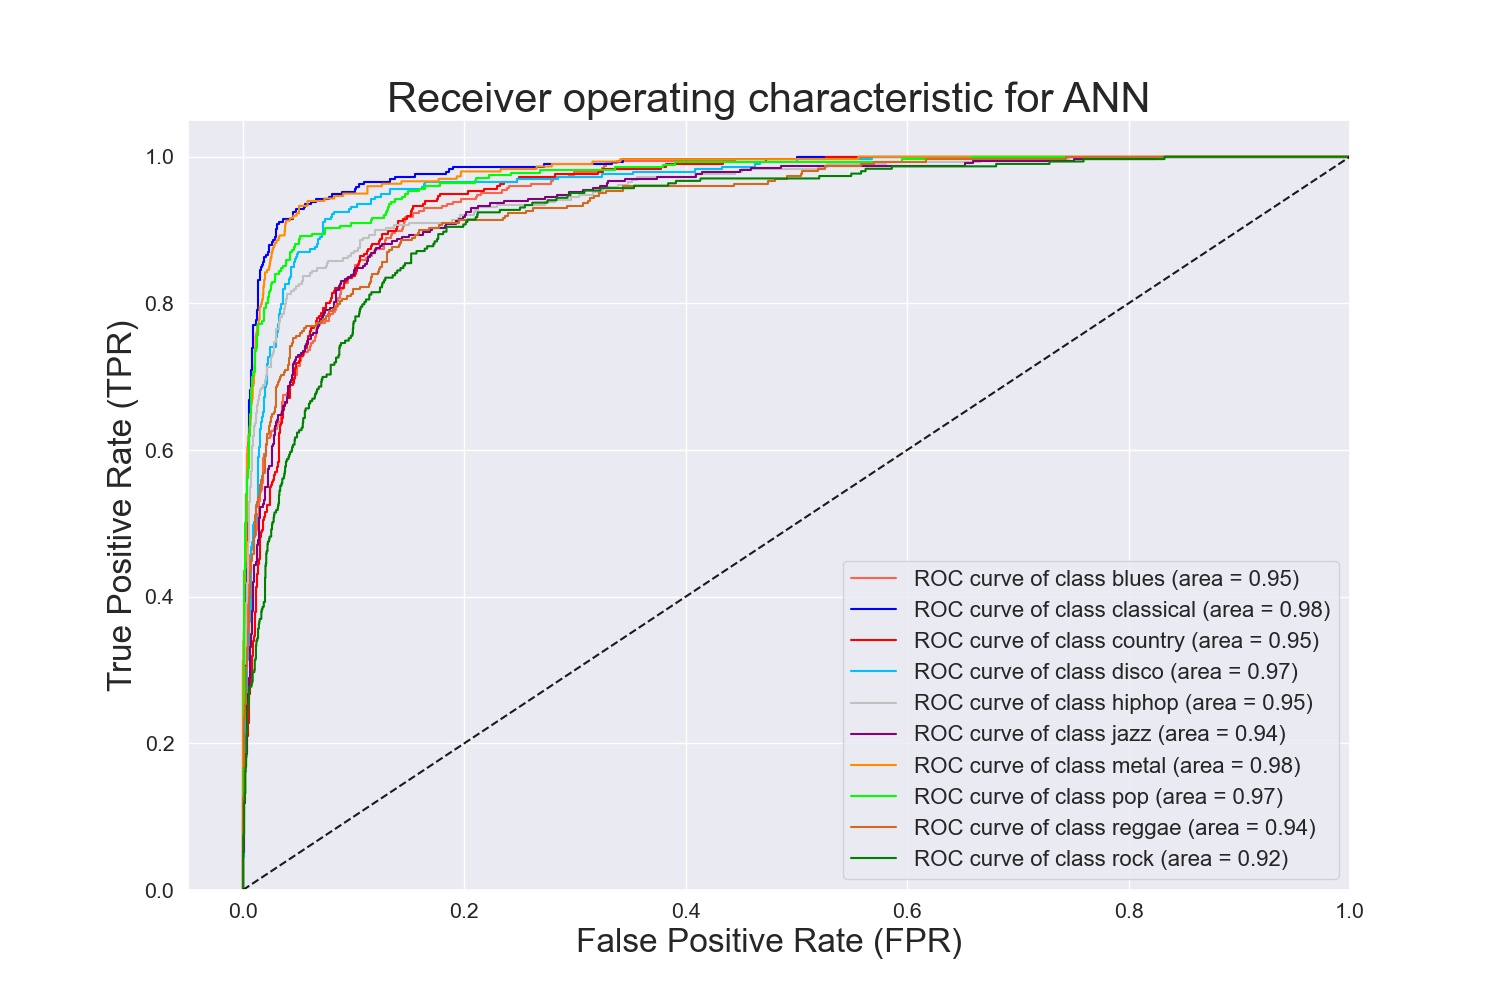
\includegraphics[width=\textwidth]{plot/SL/all_features/20/ANN_20MFCC_10000_10GEN_GTZAN - ROC Plot.jpg}
            \caption{20MFCCs ANN}
            \label{fig:20MFCCs ANN Time+frequency Features}
        \end{minipage}
        \begin{minipage}[t]{.24\textwidth}
            \centering
            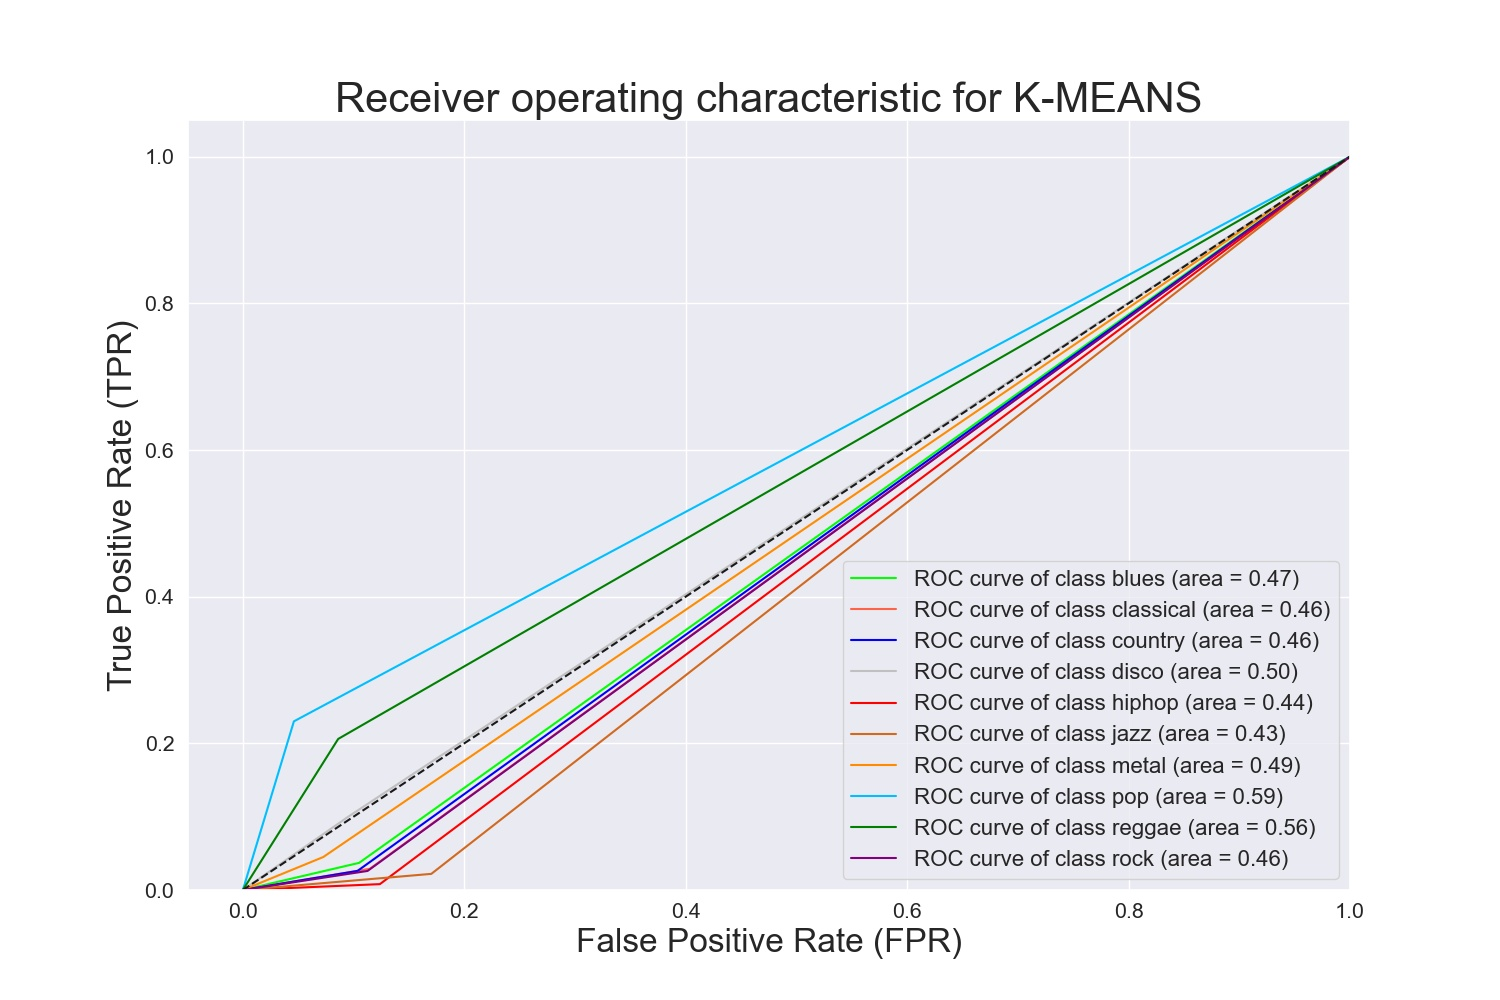
\includegraphics[width=\textwidth]{plot/UL/all_features/20/20MFCC_10000_10GEN_GTZAN - ROC Plot.jpg}
            \caption{20MFCCs K-Means}
            \label{fig:20MFCCs K-Means Time+frequency Features}
        \end{minipage}
    \end{center}
\end{figure}

\begin{table}[!ht]
    \centering
    \caption{20MFCCs supervised approach Time+frequency features}
    \label{tab:20MFCCs Time+Frequency Features Table Results}
    \begin{tabular}{c c c c c}
    \toprule
    &\multicolumn{4}{c}{20MFCCs}\\
    \cmidrule{2-5}
        Classifier  &Acc(\%) &RMSE &F1 &Ex.Time(s)\\
    \midrule 
        SVM             &60,23 &2,75 &0,59 &37,38\\
        RF              &\textcolor{orange}{\textbf{85,96}}&\textcolor{orange}{\textbf{1,59}}
                        &\textcolor{orange}{\textbf{0,85}}&\textcolor{orange}{\textbf{58,22}}\\
        ANN             &71,89 &2,33 &0,71 &310,88\\
    \bottomrule
    \end{tabular}
\end{table}

\begin{figure}[!ht]
    \begin{center}
        \small\textbf{40 MFFCs - ROC results curves for Time+frequency features}\par\medskip
        \begin{minipage}[t]{.24\textwidth}
            \centering
            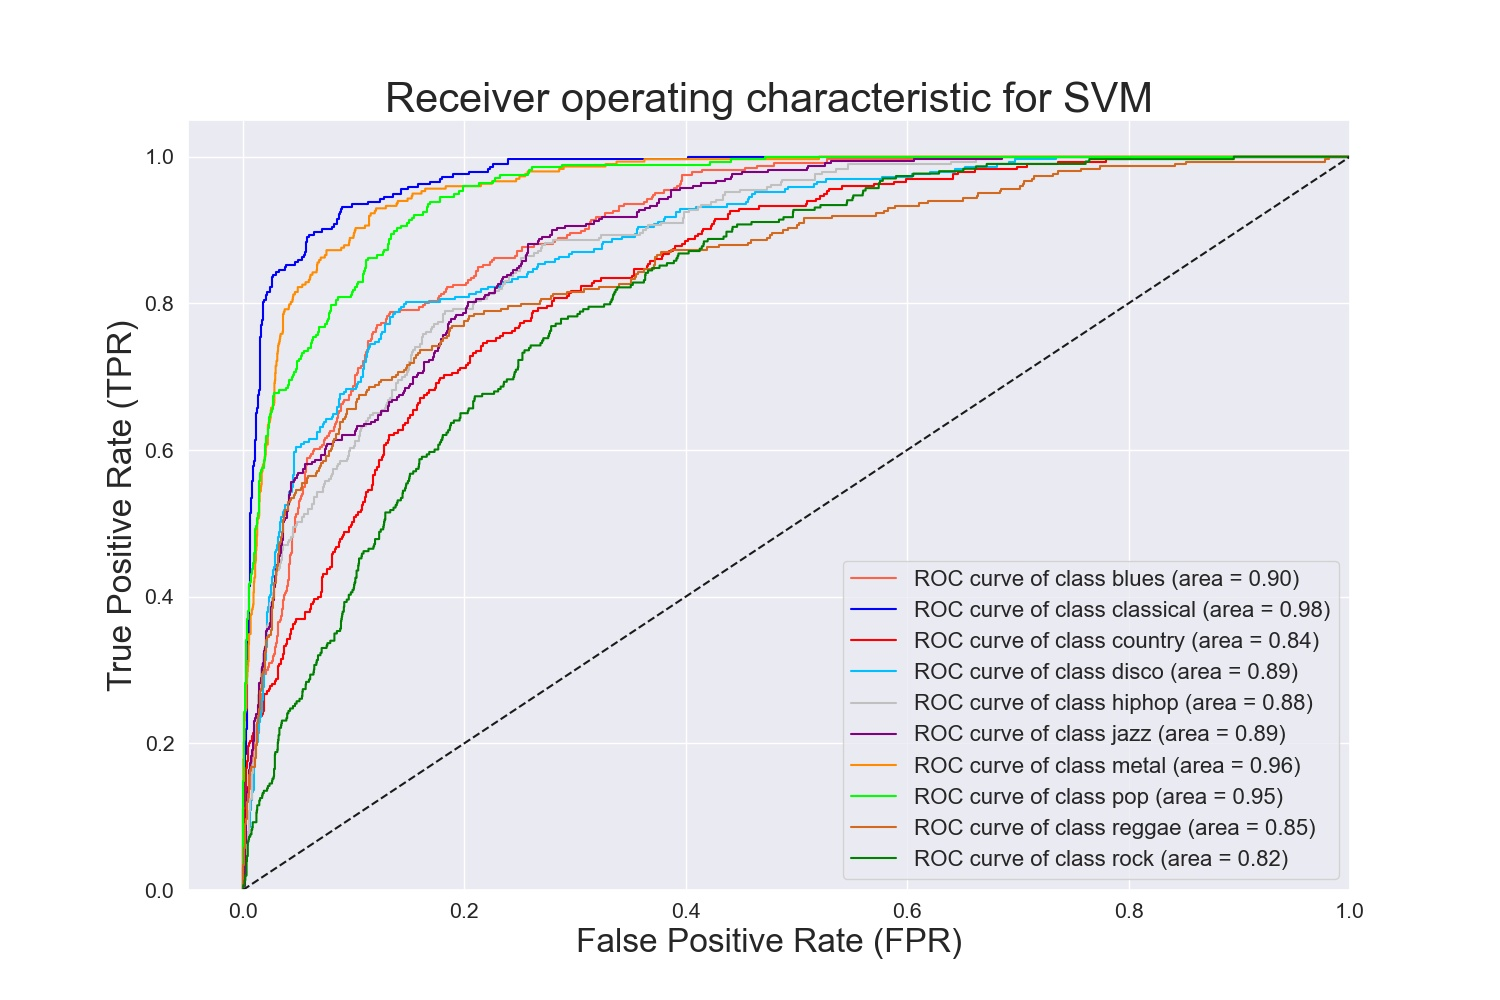
\includegraphics[width=\textwidth]{plot/SL/all_features/40/SVM_40MFCC_10000_10GEN_GTZAN - ROC Plot.jpg}
            \caption{40MFCCs SVM}
            \label{fig:40MFCCs SVM Time+frequency Features}
        \end{minipage}
        \begin{minipage}[t]{.24\textwidth}
            \centering
            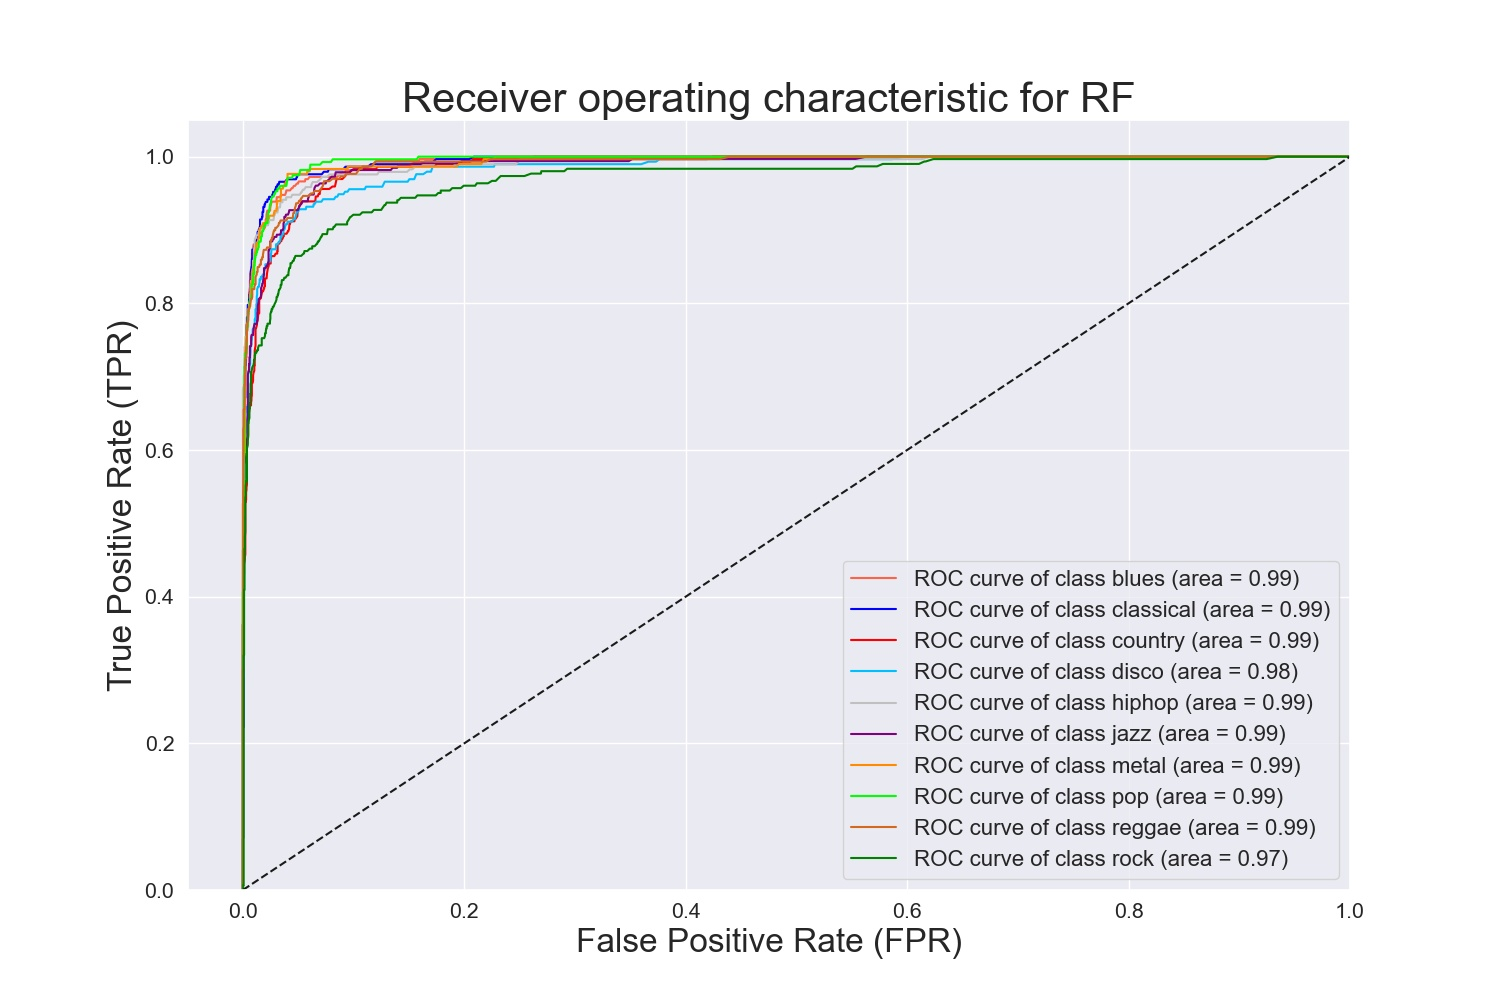
\includegraphics[width=\textwidth]{plot/SL/all_features/40/RF_40MFCC_10000_10GEN_GTZAN - ROC Plot.jpg}
            \caption{40MFCCs RF}
            \label{fig:40MFCCs RF Time+frequency Features}
        \end{minipage}
        \begin{minipage}[t]{.24\textwidth}
            \centering
            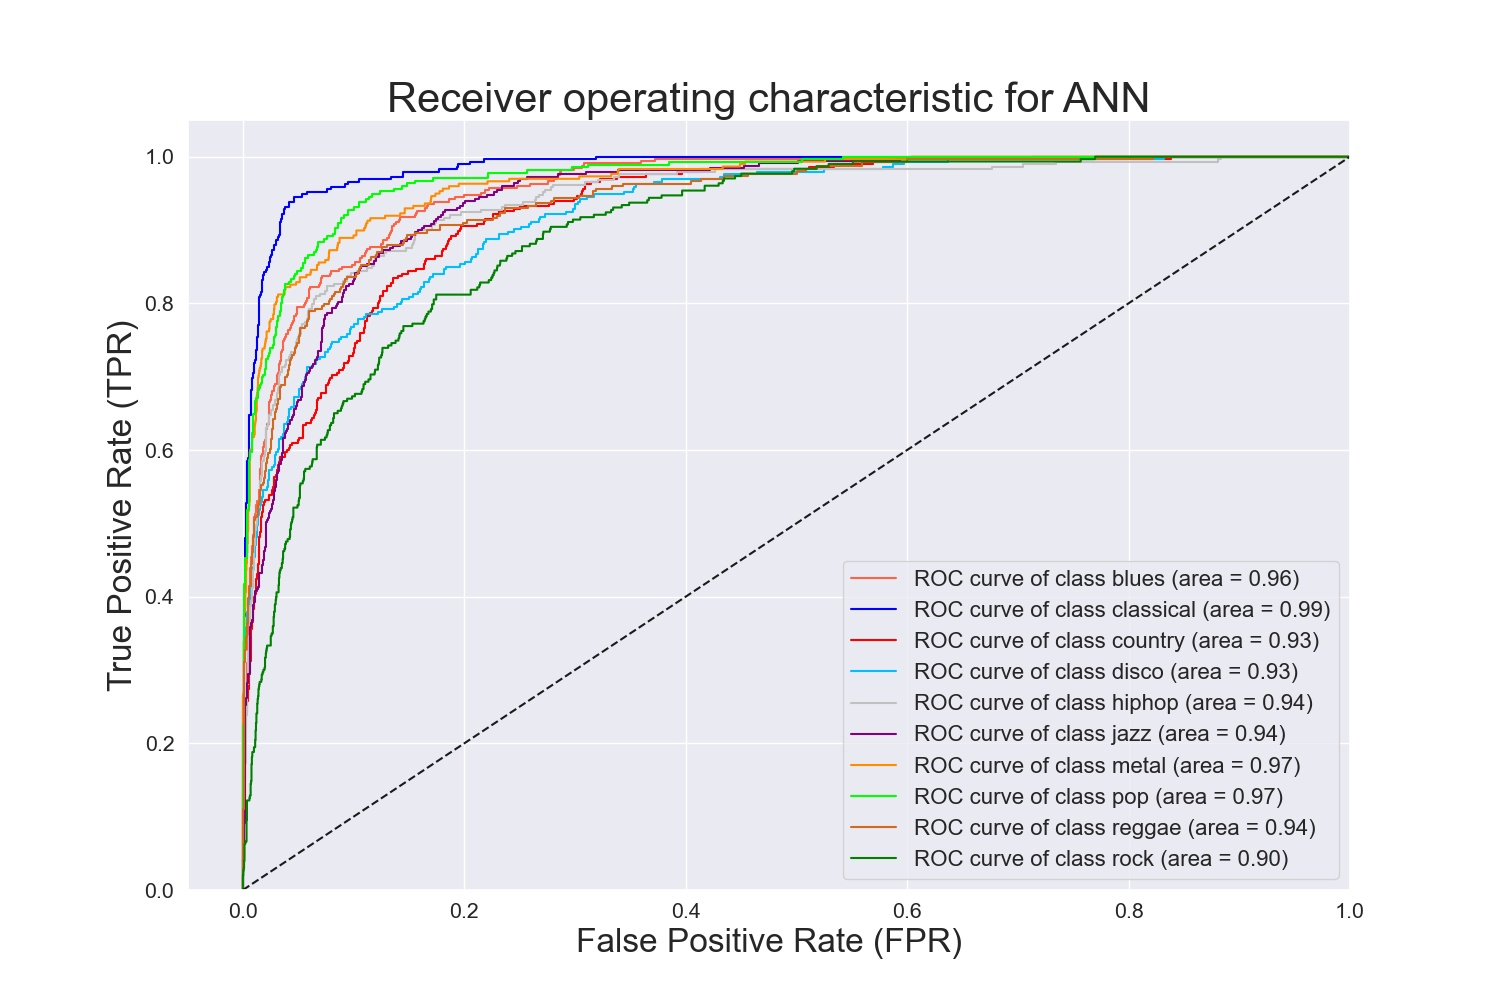
\includegraphics[width=\textwidth]{plot/SL/all_features/40/ANN_40MFCC_10000_10GEN_GTZAN - ROC Plot.jpg}
            \caption{40MFCCs ANN}
            \label{fig:40MFCCs ANN Time+frequency Features}
        \end{minipage}
        \begin{minipage}[t]{.24\textwidth}
            \centering
            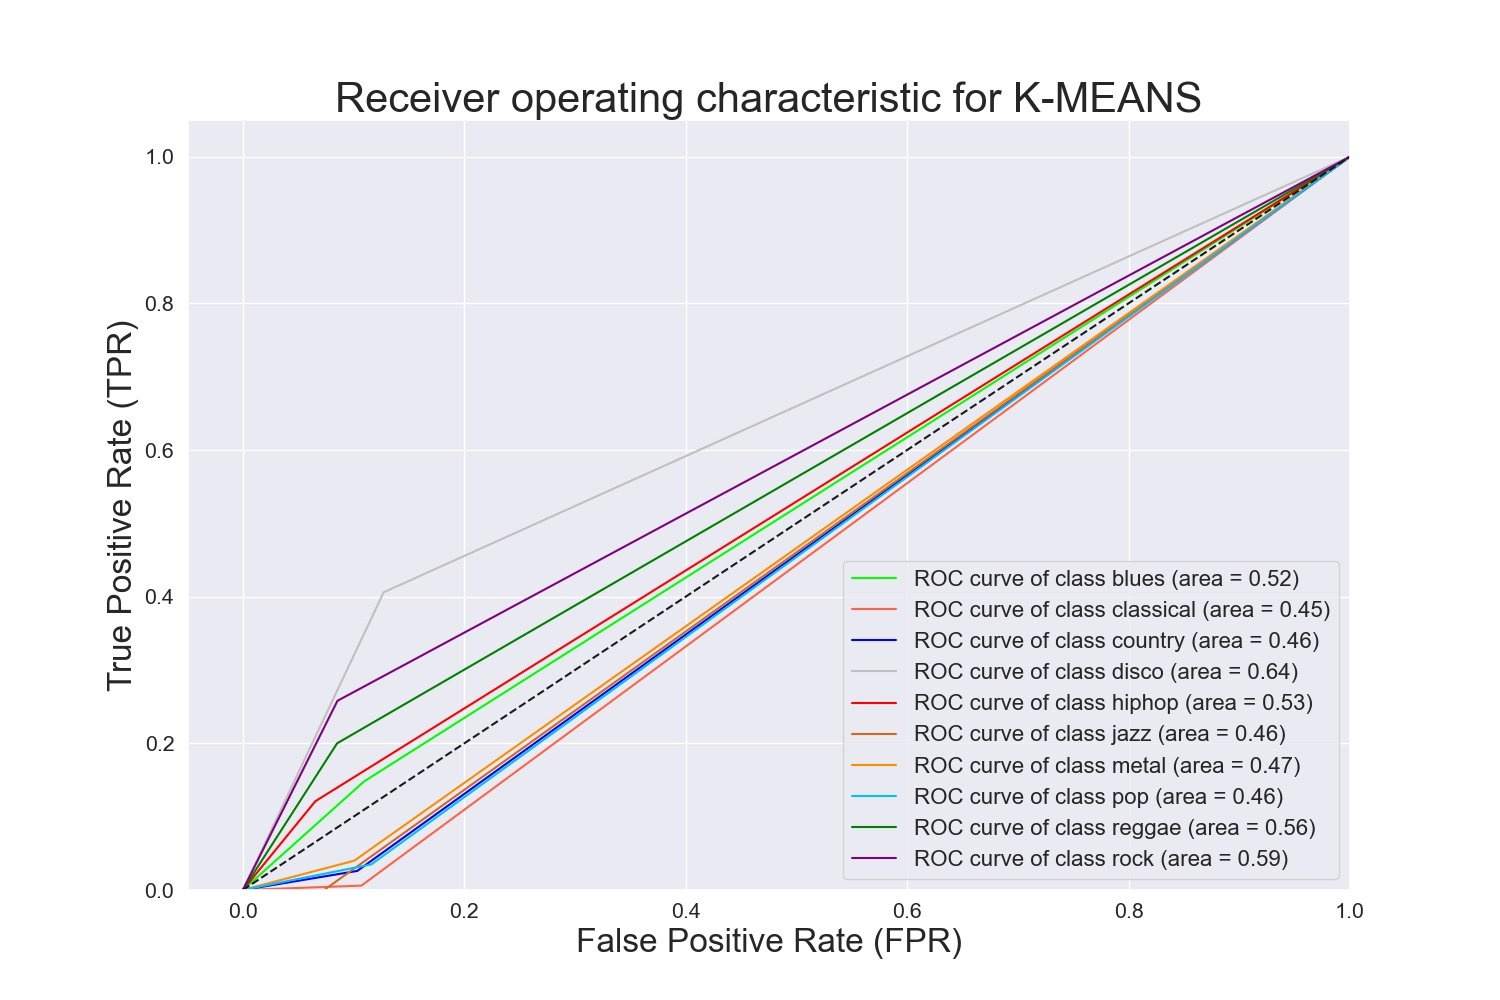
\includegraphics[width=\textwidth]{plot/UL/all_features/40/40MFCC_10000_10GEN_GTZAN - ROC Plot.jpg}
            \caption{40MFCCs K-Means}
            \label{fig:40MFCCs K-Means Time+frequency Features}
        \end{minipage}
    \end{center}
\end{figure}

\begin{table}[!ht]
    \centering
    \caption{40MFCCs supervised approach Time+frequency features}
    \label{tab:40MFCCs Time+Frequency Features Table Results}
    \begin{tabular}{c c c c c}
    \toprule
    &\multicolumn{4}{c}{40MFCCs}\\
    \cmidrule{2-5}
        Classifier  &Acc(\%) &RMSE &F1 &Ex.Time(s)\\
    \midrule 
        SVM             &57,83 &2,77 &0,56 &40,68\\    
        RF              &\textcolor{green}{\textbf{86,06}}&\textcolor{green}{\textbf{1,52}}
                        &\textcolor{green}{\textbf{0,86}}&\textcolor{green}{\textbf{72,40}}\\
        ANN             &67,13 &2,40 &0,66 &335,67\\
    \bottomrule
    \end{tabular}
\end{table}

\section{Conclusions And Future Work}
\noindent
In this article it was possible to prove how the increase of features isn't always the best solution. It's possible to see how the optimal result considered, taking into account costs and benefits is that with 20 MFCCs (Tab. \ref{tab:20MFCCs Time+Frequency Features Table Results}). Although the table relating to 40 MFCCs (Tab. \ref{tab:40MFCCs Time+Frequency Features Table Results} contains slightly higher values, the execution time and above all the time used for the realization of the data sets isn't worth the obtained benefit. Also as regards the classifiers, the most used ones aren't always the best, or in any case they can achieve the same performance but with a greater increase in execution time. In fact, with a lot of probability it's possible to reach close values obtained in Tab. \ref{tab:20MFCCs Time+Frequency Features Table Results} by adding neurons, modifying the topology of the neural network and and performing a very thorough tuning, going however to meet a greater computational complexity and a higher execution time. Another point of attention is related to the unsupervised approach, we have been able to see how the high number of features, with values very close to each other, do not allow the algorithm to be able to cluster optimally while keeping high the inter cluster distance. Future developments are related to the search for efficient methods of selecting the most relevant features for the unsupervised approach, the use of new classification algorithms or networks already known such as CNN that can be used by directly passing the extracted images of Mel-Spectrogram or Log-Mel Spectrogram.

\noindent
\bibliographystyle{IEEEtran}
\bibliography{references}
\end{document}
